\chapter{Appendix}

\section{Line Candidate Cutouts}\label{sec:A1}

The following plots show the 35 CO line candidates in various wavelengths. The red contours show the +2$\sigma$,4$\sigma$, and 6$\sigma$ values in the datacubes. All cutouts are 3x3 arcseconds in size.

\begin{figure}[tbp]
\centering 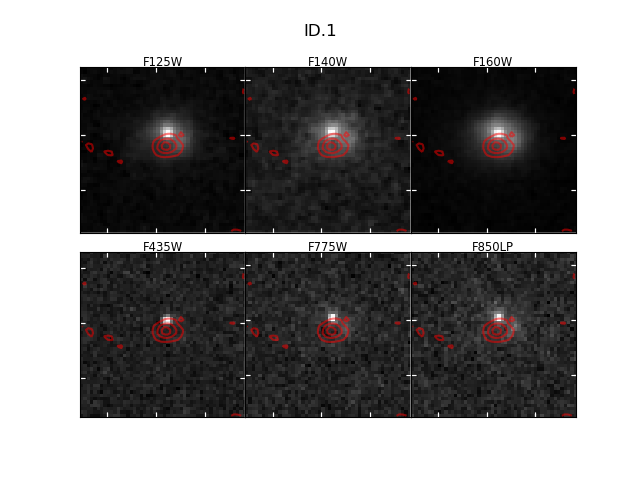
\includegraphics[width=160mm]{Matched/ASPECS_Cutout_0.png}
\caption{ID.1. Red contours signify +2$\sigma$,4$\sigma$, and 6$\sigma$. The size of the cutouts are 3x3 arcseconds. The spacing between the ticks is one arcsecond.}
\label{fig:Match_One}
\end{figure}

\begin{figure}[tbp]
\centering 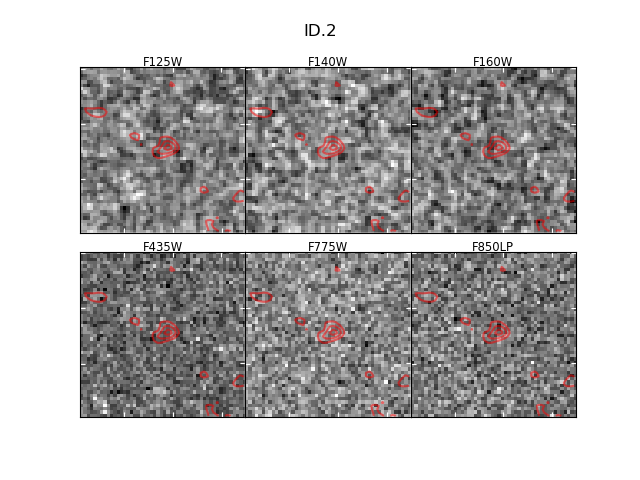
\includegraphics[width=160mm]{Matched/ASPECS_Cutout_1.png}
\caption{ID.2. Same contours and cutout size as for \ref{fig:Match_One}.}
\label{fig:Match_Two}
\end{figure}


\begin{figure}[tbp]
\centering 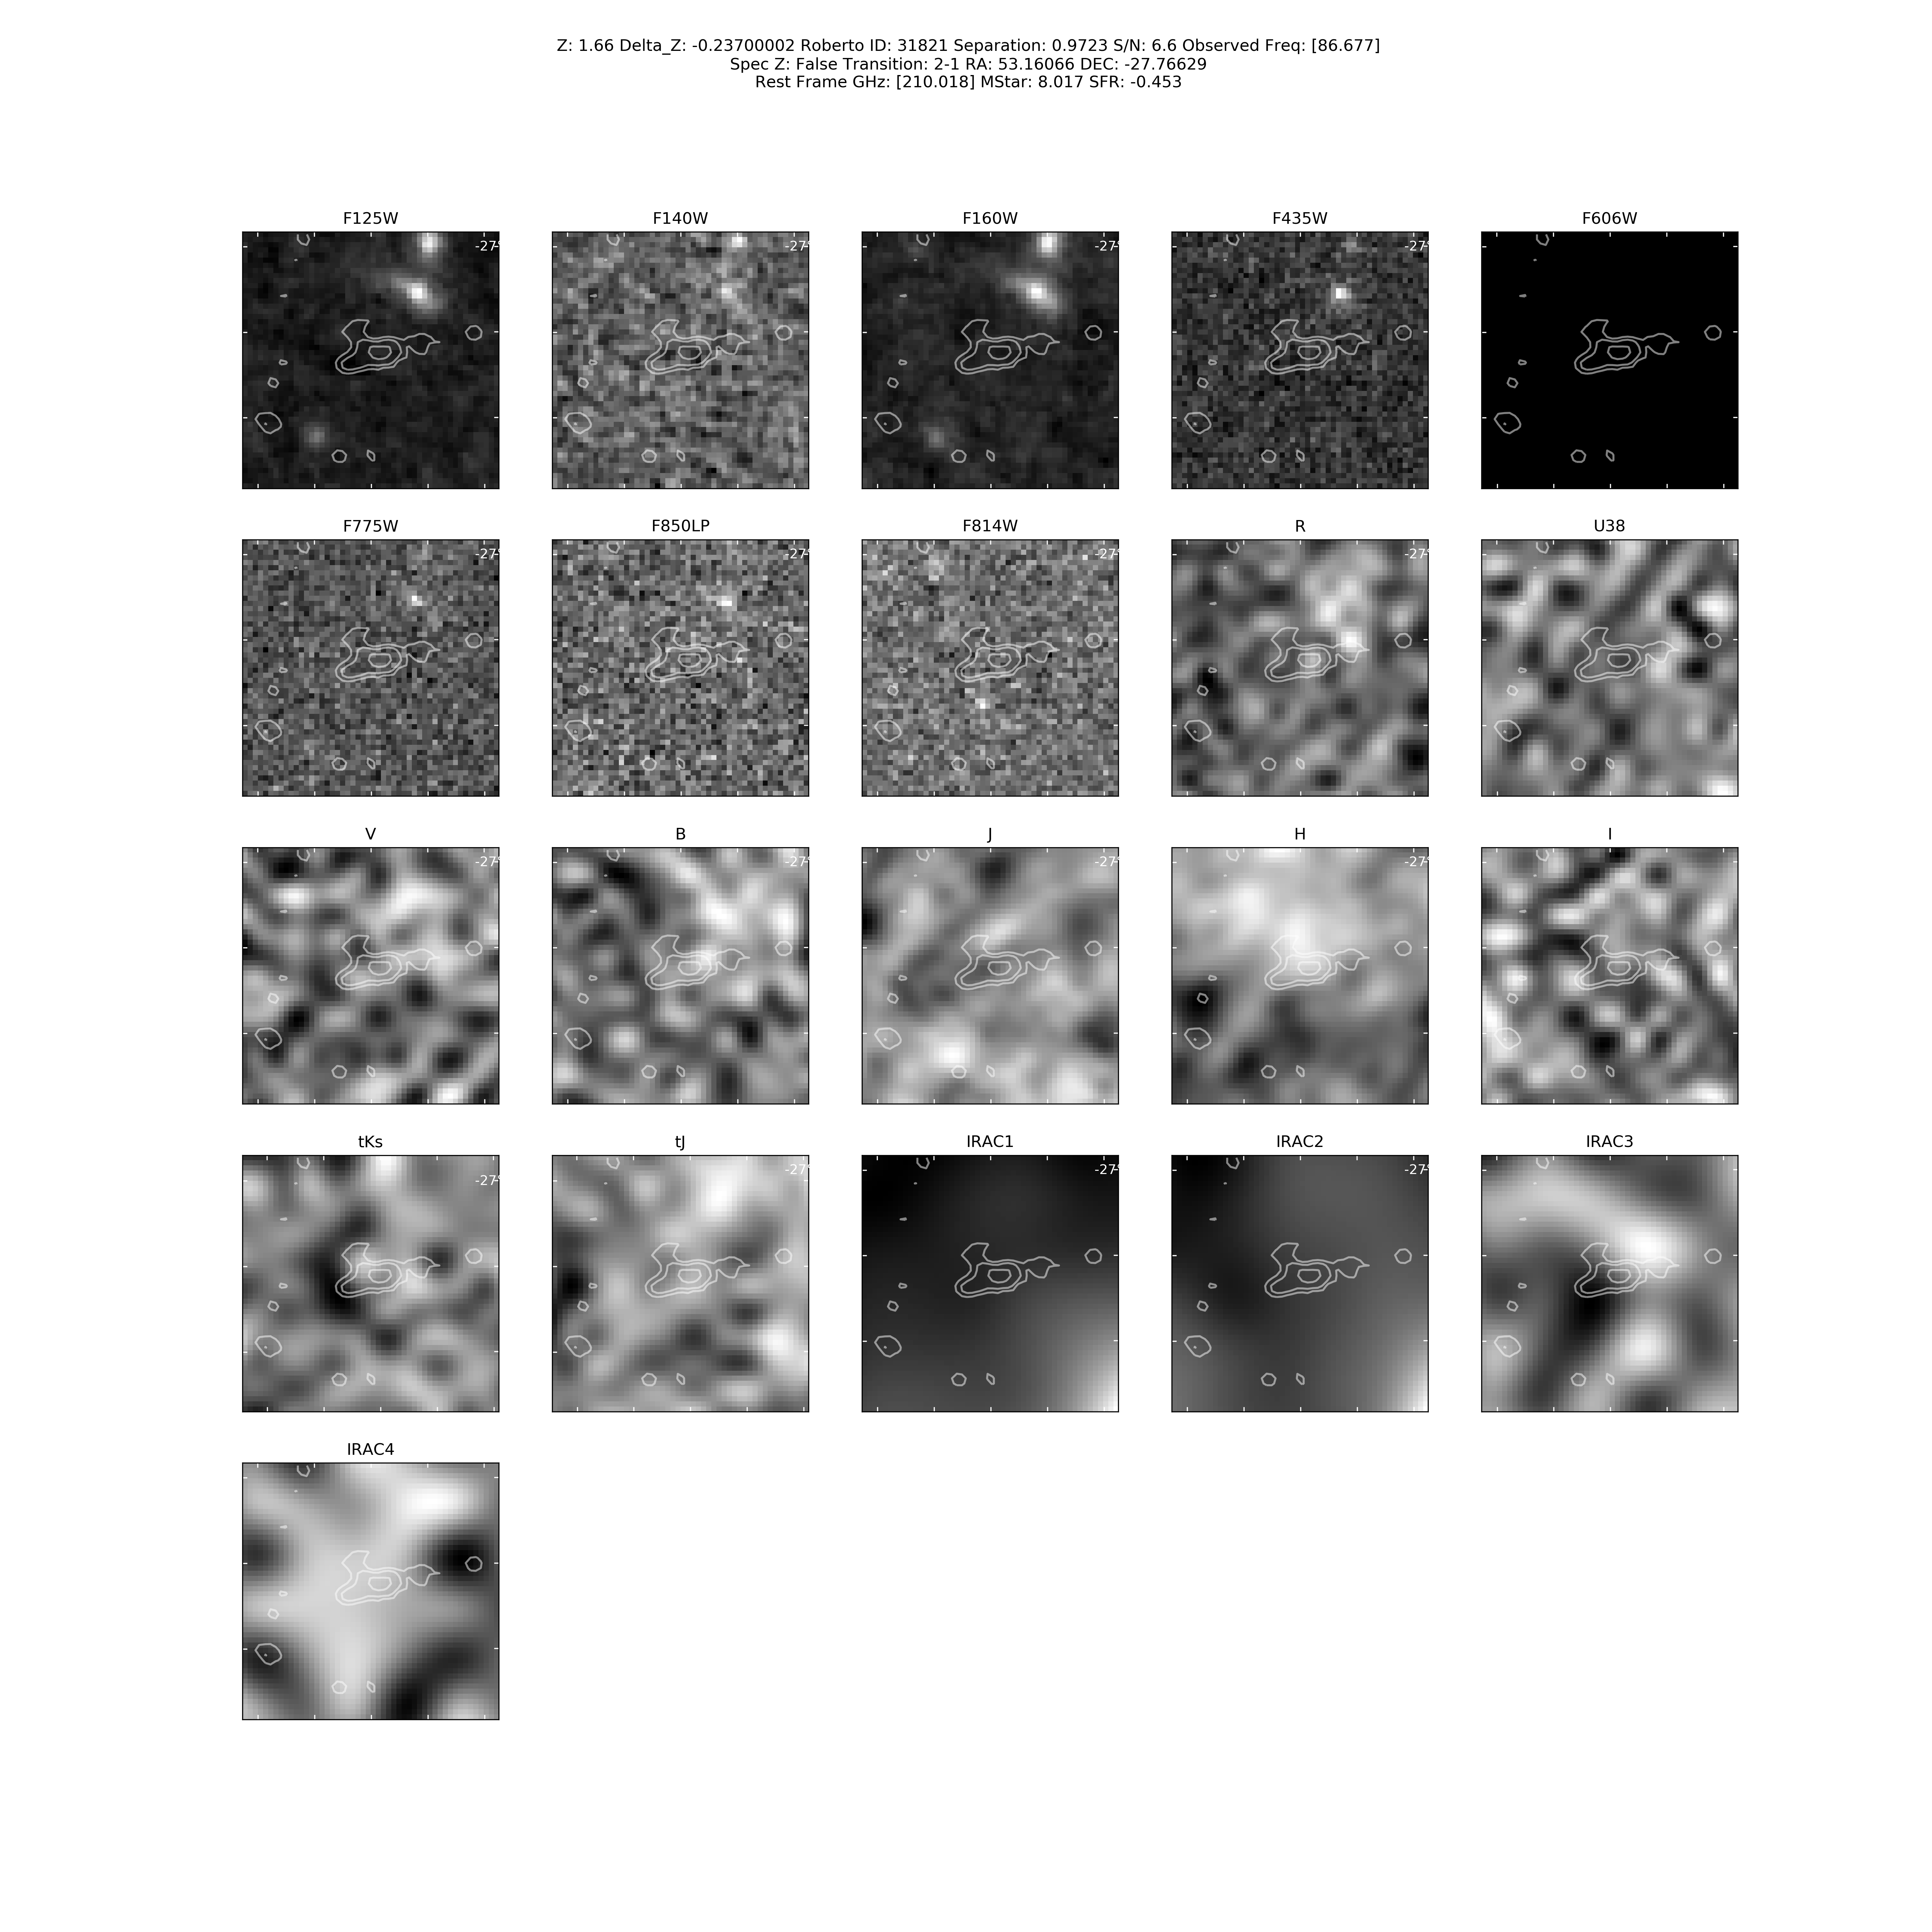
\includegraphics[width=160mm]{Matched/ASPECS_Cutout_2.png}
\caption{ID.3. Same contours and cutout size as for \ref{fig:Match_One}.}
\label{fig:Match_Three}
\end{figure}

\begin{figure}[tbp]
\centering 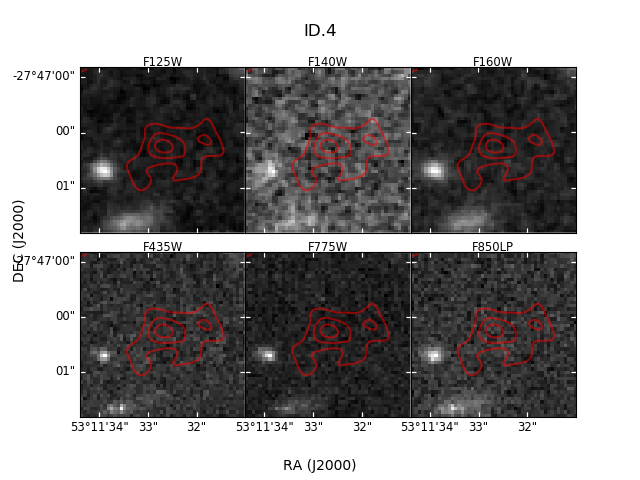
\includegraphics[width=160mm]{Matched/ASPECS_Cutout_3.png}
\caption{ID.4. Same contours and cutout size as for \ref{fig:Match_One}.}
\label{fig:Match_Three}
\end{figure}

\begin{figure}[tbp]
\centering 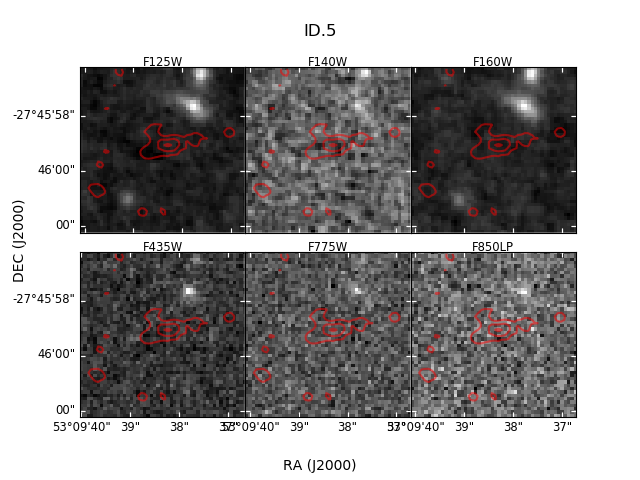
\includegraphics[width=160mm]{Matched/ASPECS_Cutout_4.png}
\caption{ID.5. Same contours and cutout size as for \ref{fig:Match_One}.}
\label{fig:Match_Four}
\end{figure}

\begin{figure}[tbp]
\centering 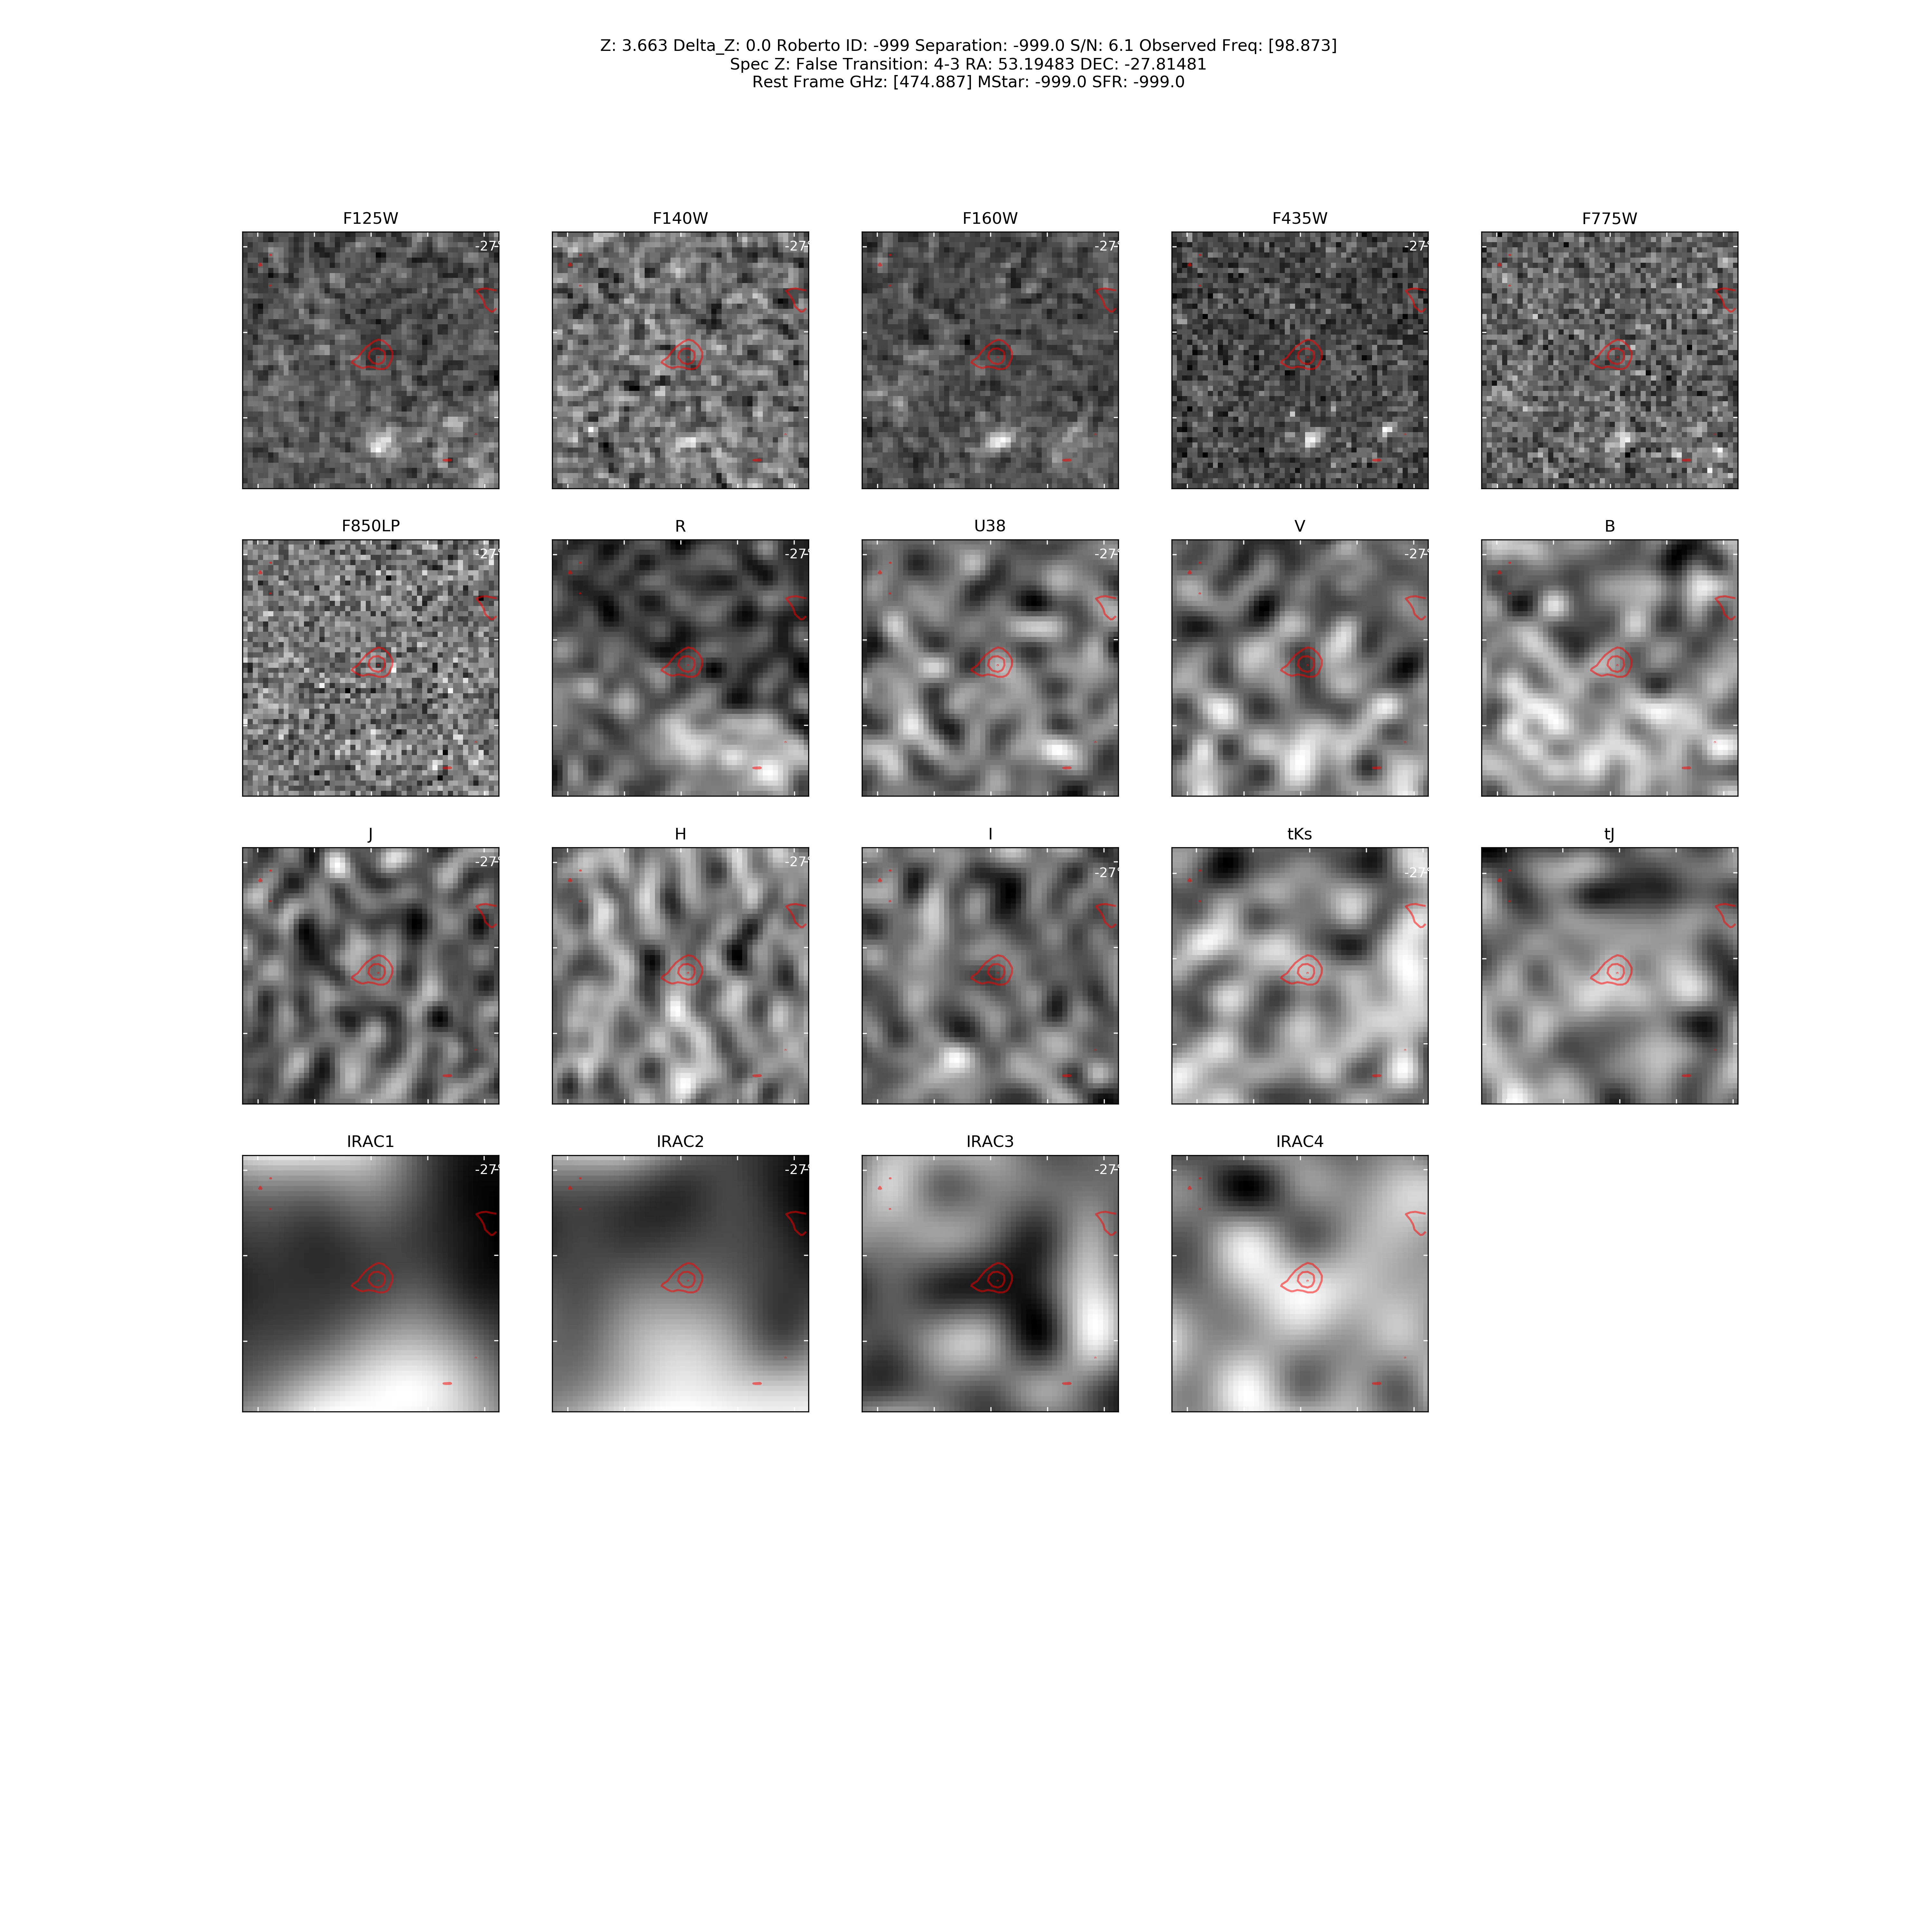
\includegraphics[width=160mm]{Matched/ASPECS_Cutout_5.png}
\caption{ID.6. Same contours and cutout size as for \ref{fig:Match_One}.}
\label{fig:Match_Five}
\end{figure}

\begin{figure}[tbp]
\centering 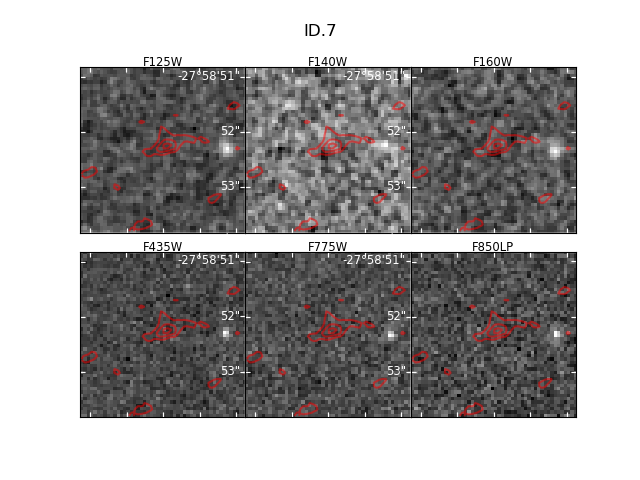
\includegraphics[width=160mm]{Matched/ASPECS_Cutout_6.png}
\caption{ID.7. Same contours and cutout size as for \ref{fig:Match_One}.}
\label{fig:Match_Three}
\end{figure}

\begin{figure}[tbp]
\centering 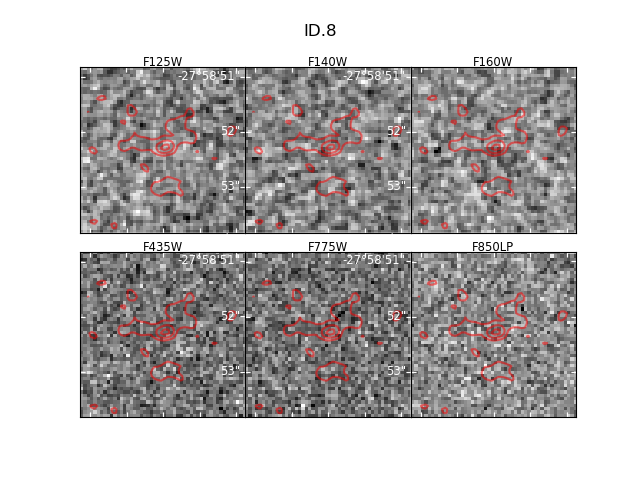
\includegraphics[width=160mm]{Matched/ASPECS_Cutout_7.png}
\caption{ID.8. Same contours and cutout size as for \ref{fig:Match_One}.}
\label{fig:Match_Three}
\end{figure}

\begin{figure}[tbp]
\centering 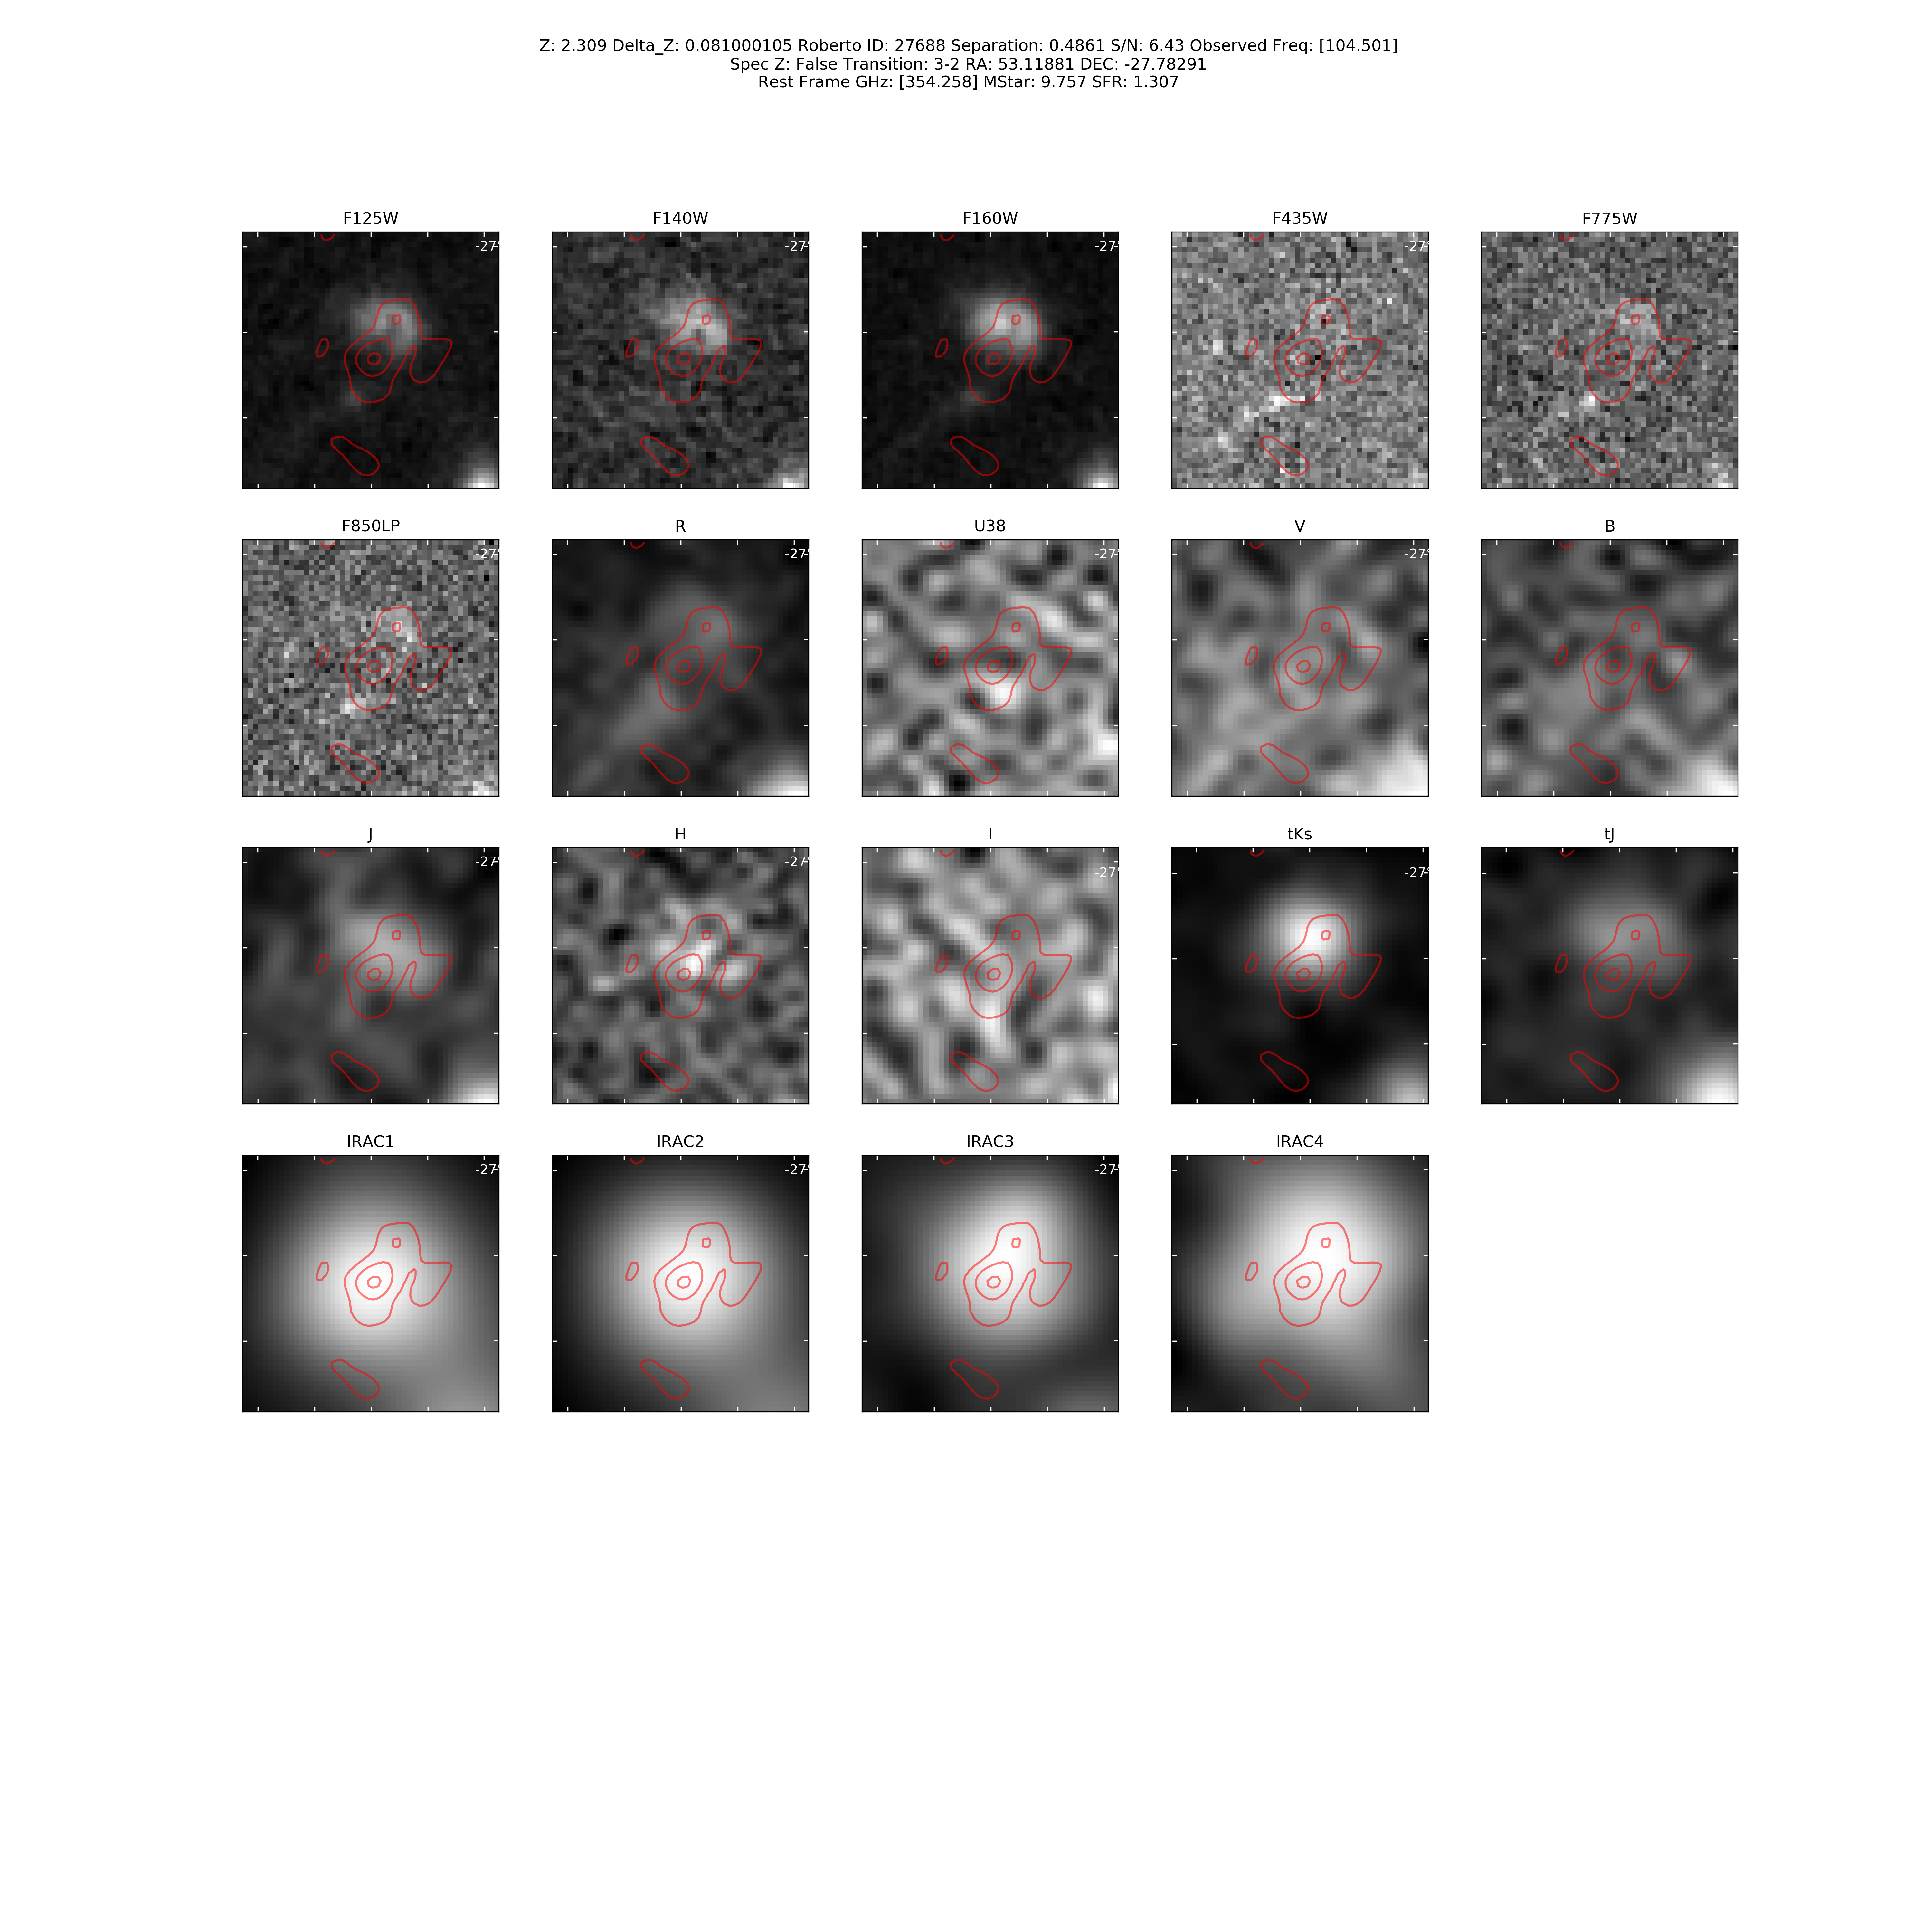
\includegraphics[width=160mm]{Matched/ASPECS_Cutout_8.png}
\caption{ID.9. Same contours and cutout size as for \ref{fig:Match_One}.}
\label{fig:Match_Three}
\end{figure}

\begin{figure}[tbp]
\centering 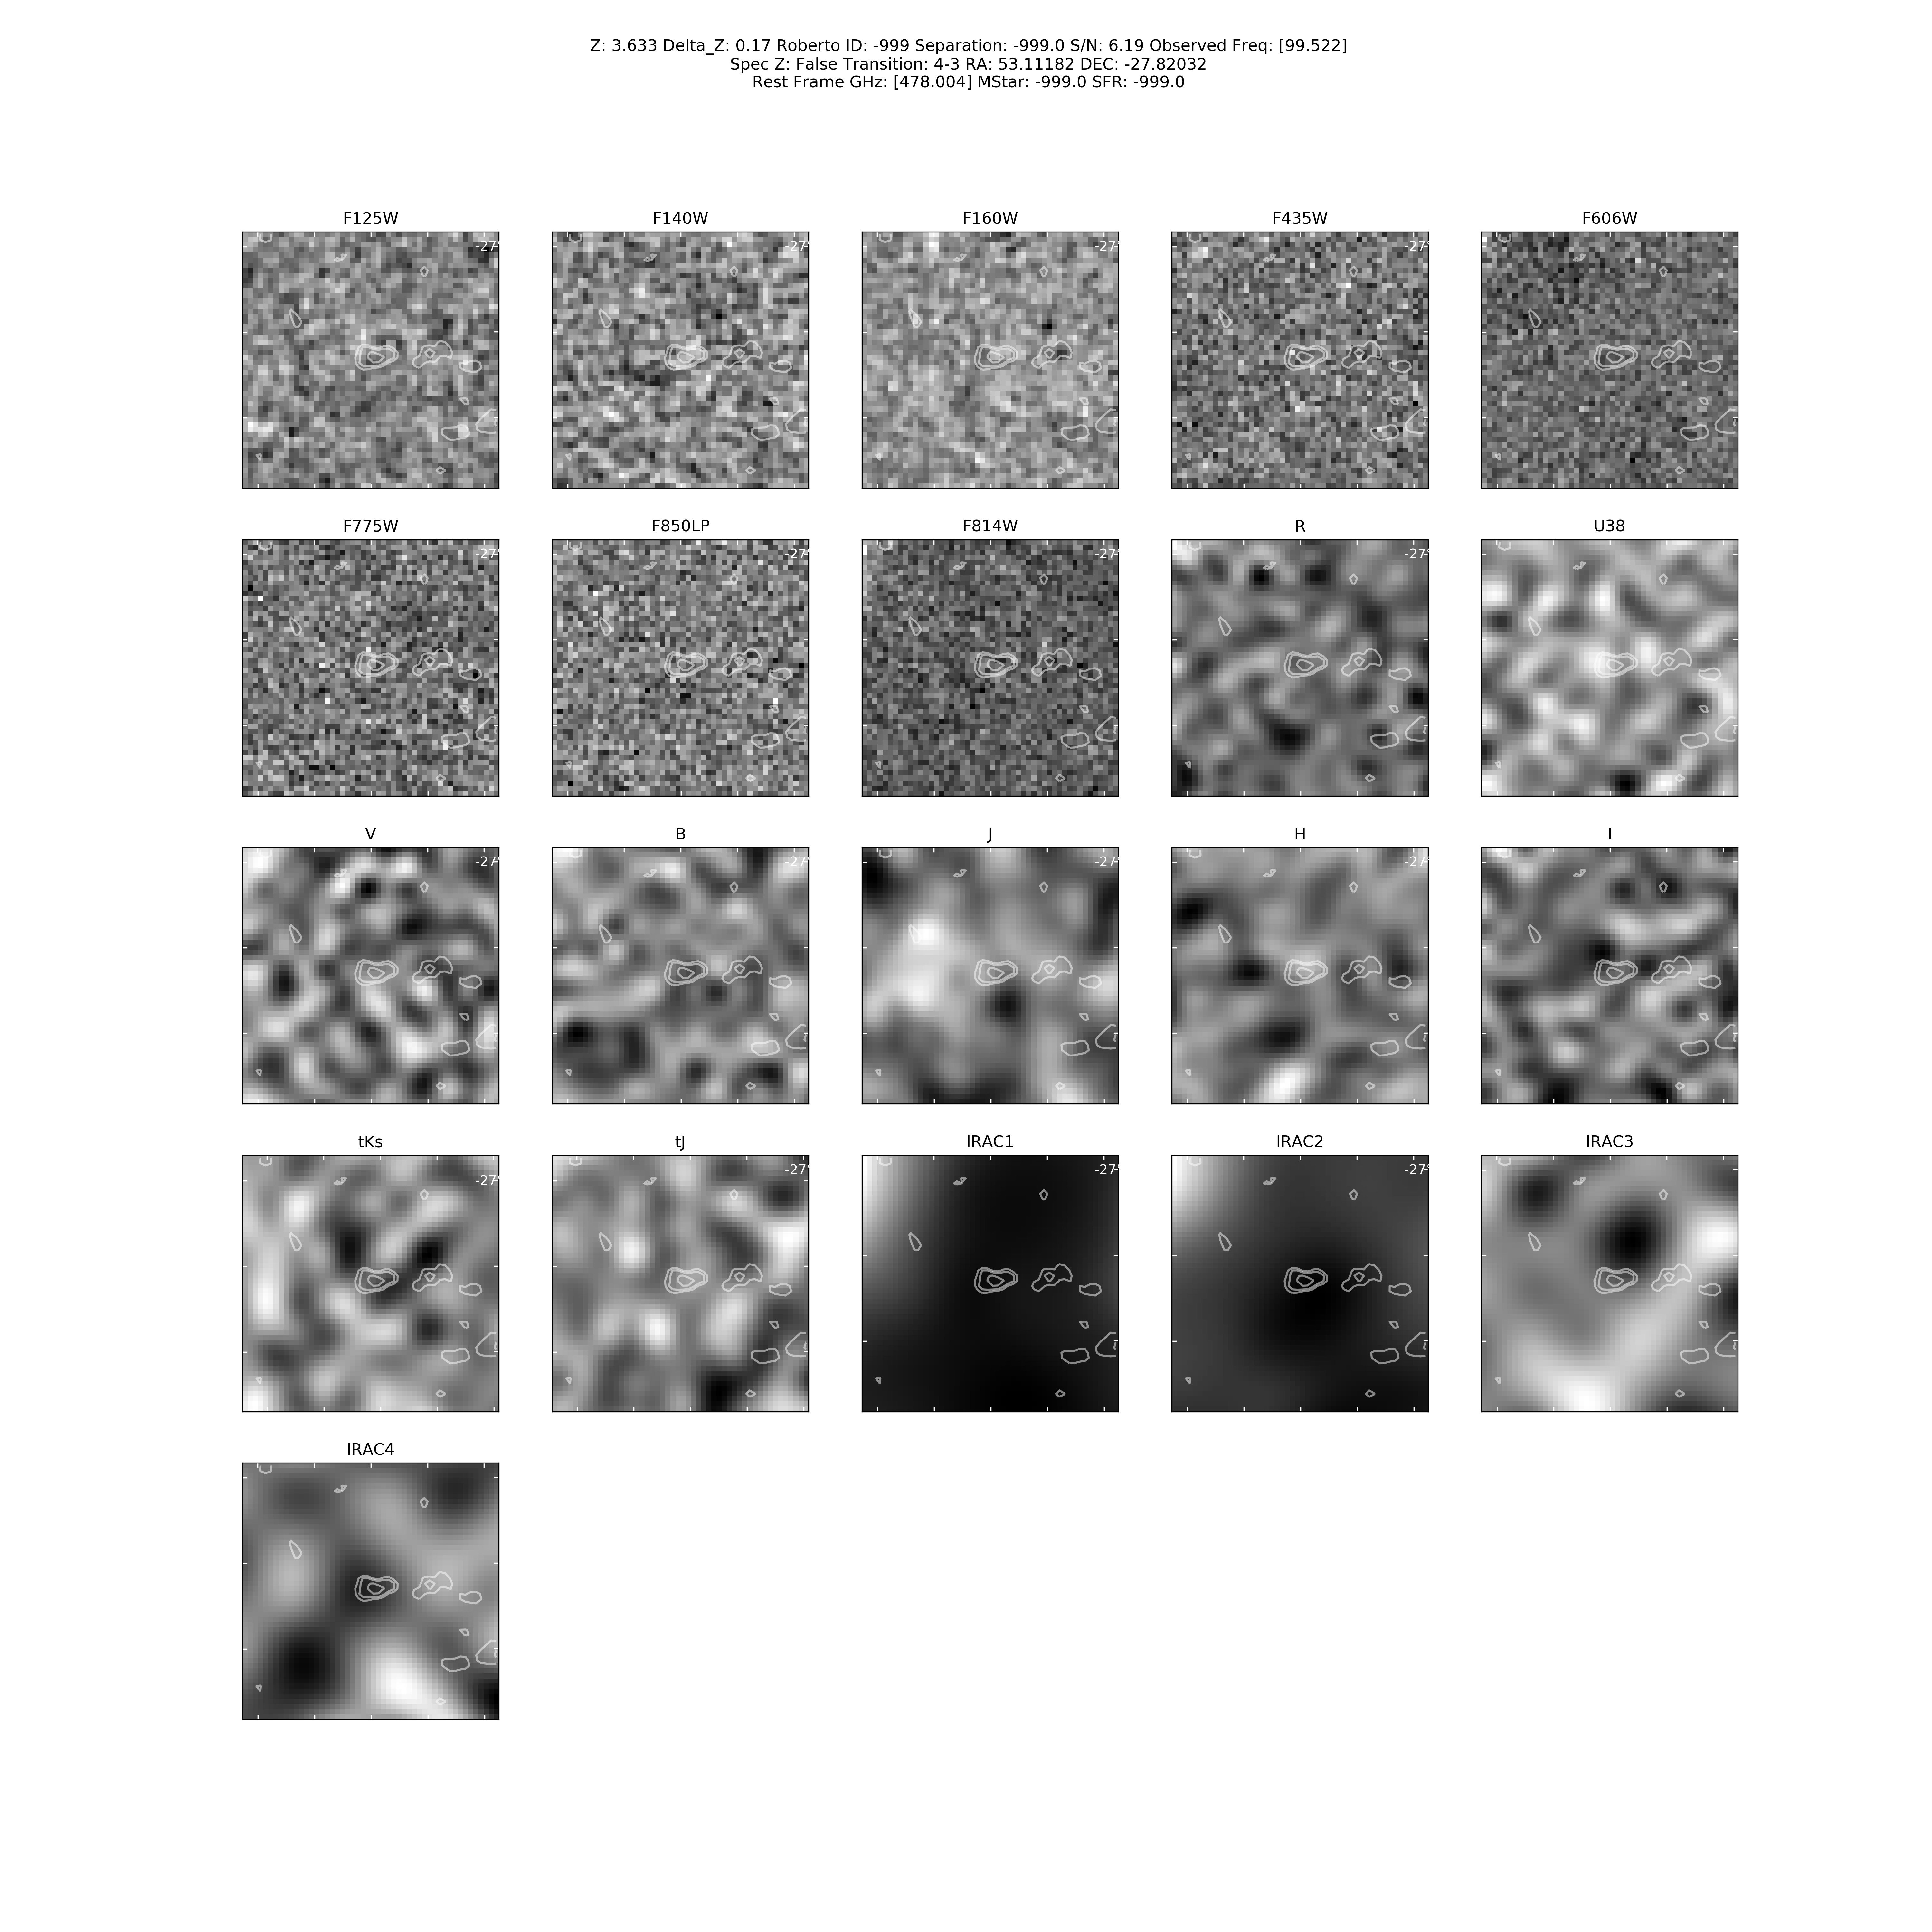
\includegraphics[width=160mm]{Matched/ASPECS_Cutout_9.png}
\caption{ID.10. Same contours and cutout size as for \ref{fig:Match_One}.}
\label{fig:Match_Three}
\end{figure}


\begin{figure}[tbp]
\centering 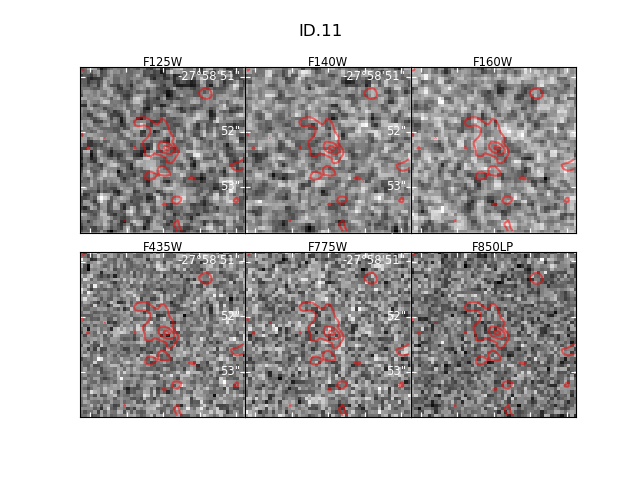
\includegraphics[width=160mm]{Matched/ASPECS_Cutout_10.png}
\caption{ID.11. Same contours and cutout size as for \ref{fig:Match_One}.}
\label{fig:Match_Three}
\end{figure}

\begin{figure}[tbp]
\centering 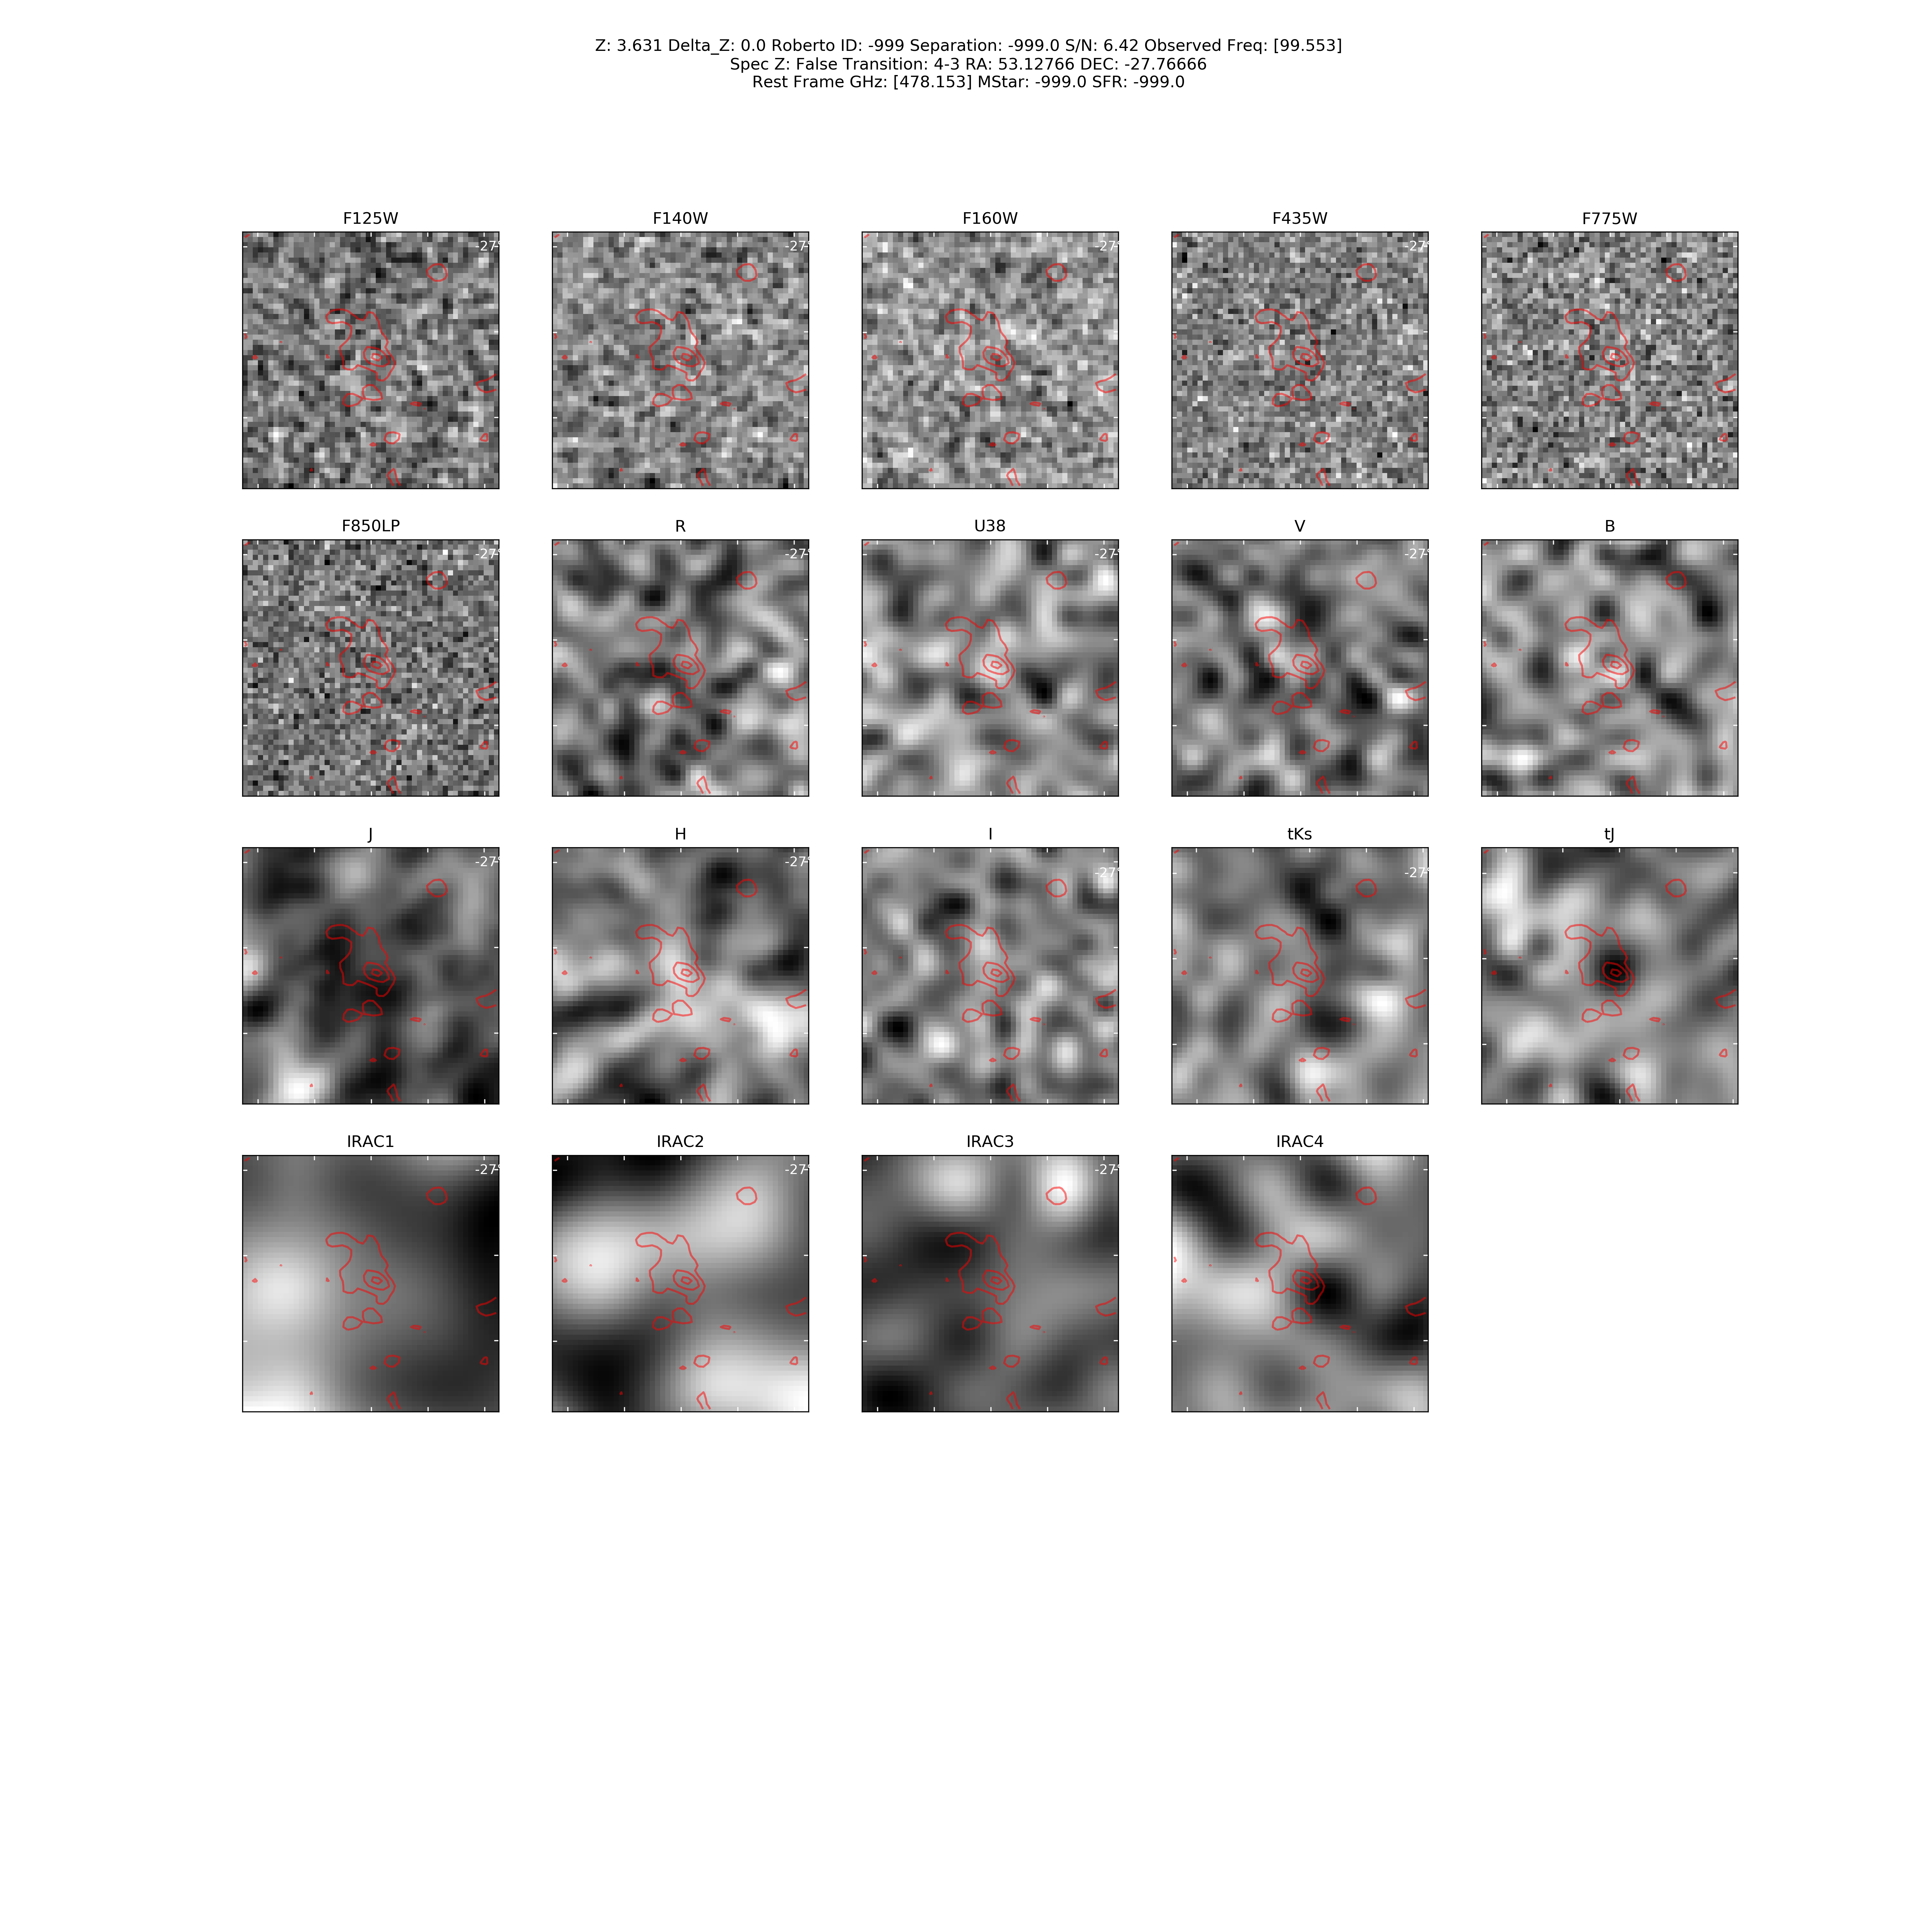
\includegraphics[width=160mm]{Matched/ASPECS_Cutout_11.png}
\caption{ID.12. Same contours and cutout size as for \ref{fig:Match_One}.}
\label{fig:Match_Three}
\end{figure}

\begin{figure}[tbp]
\centering 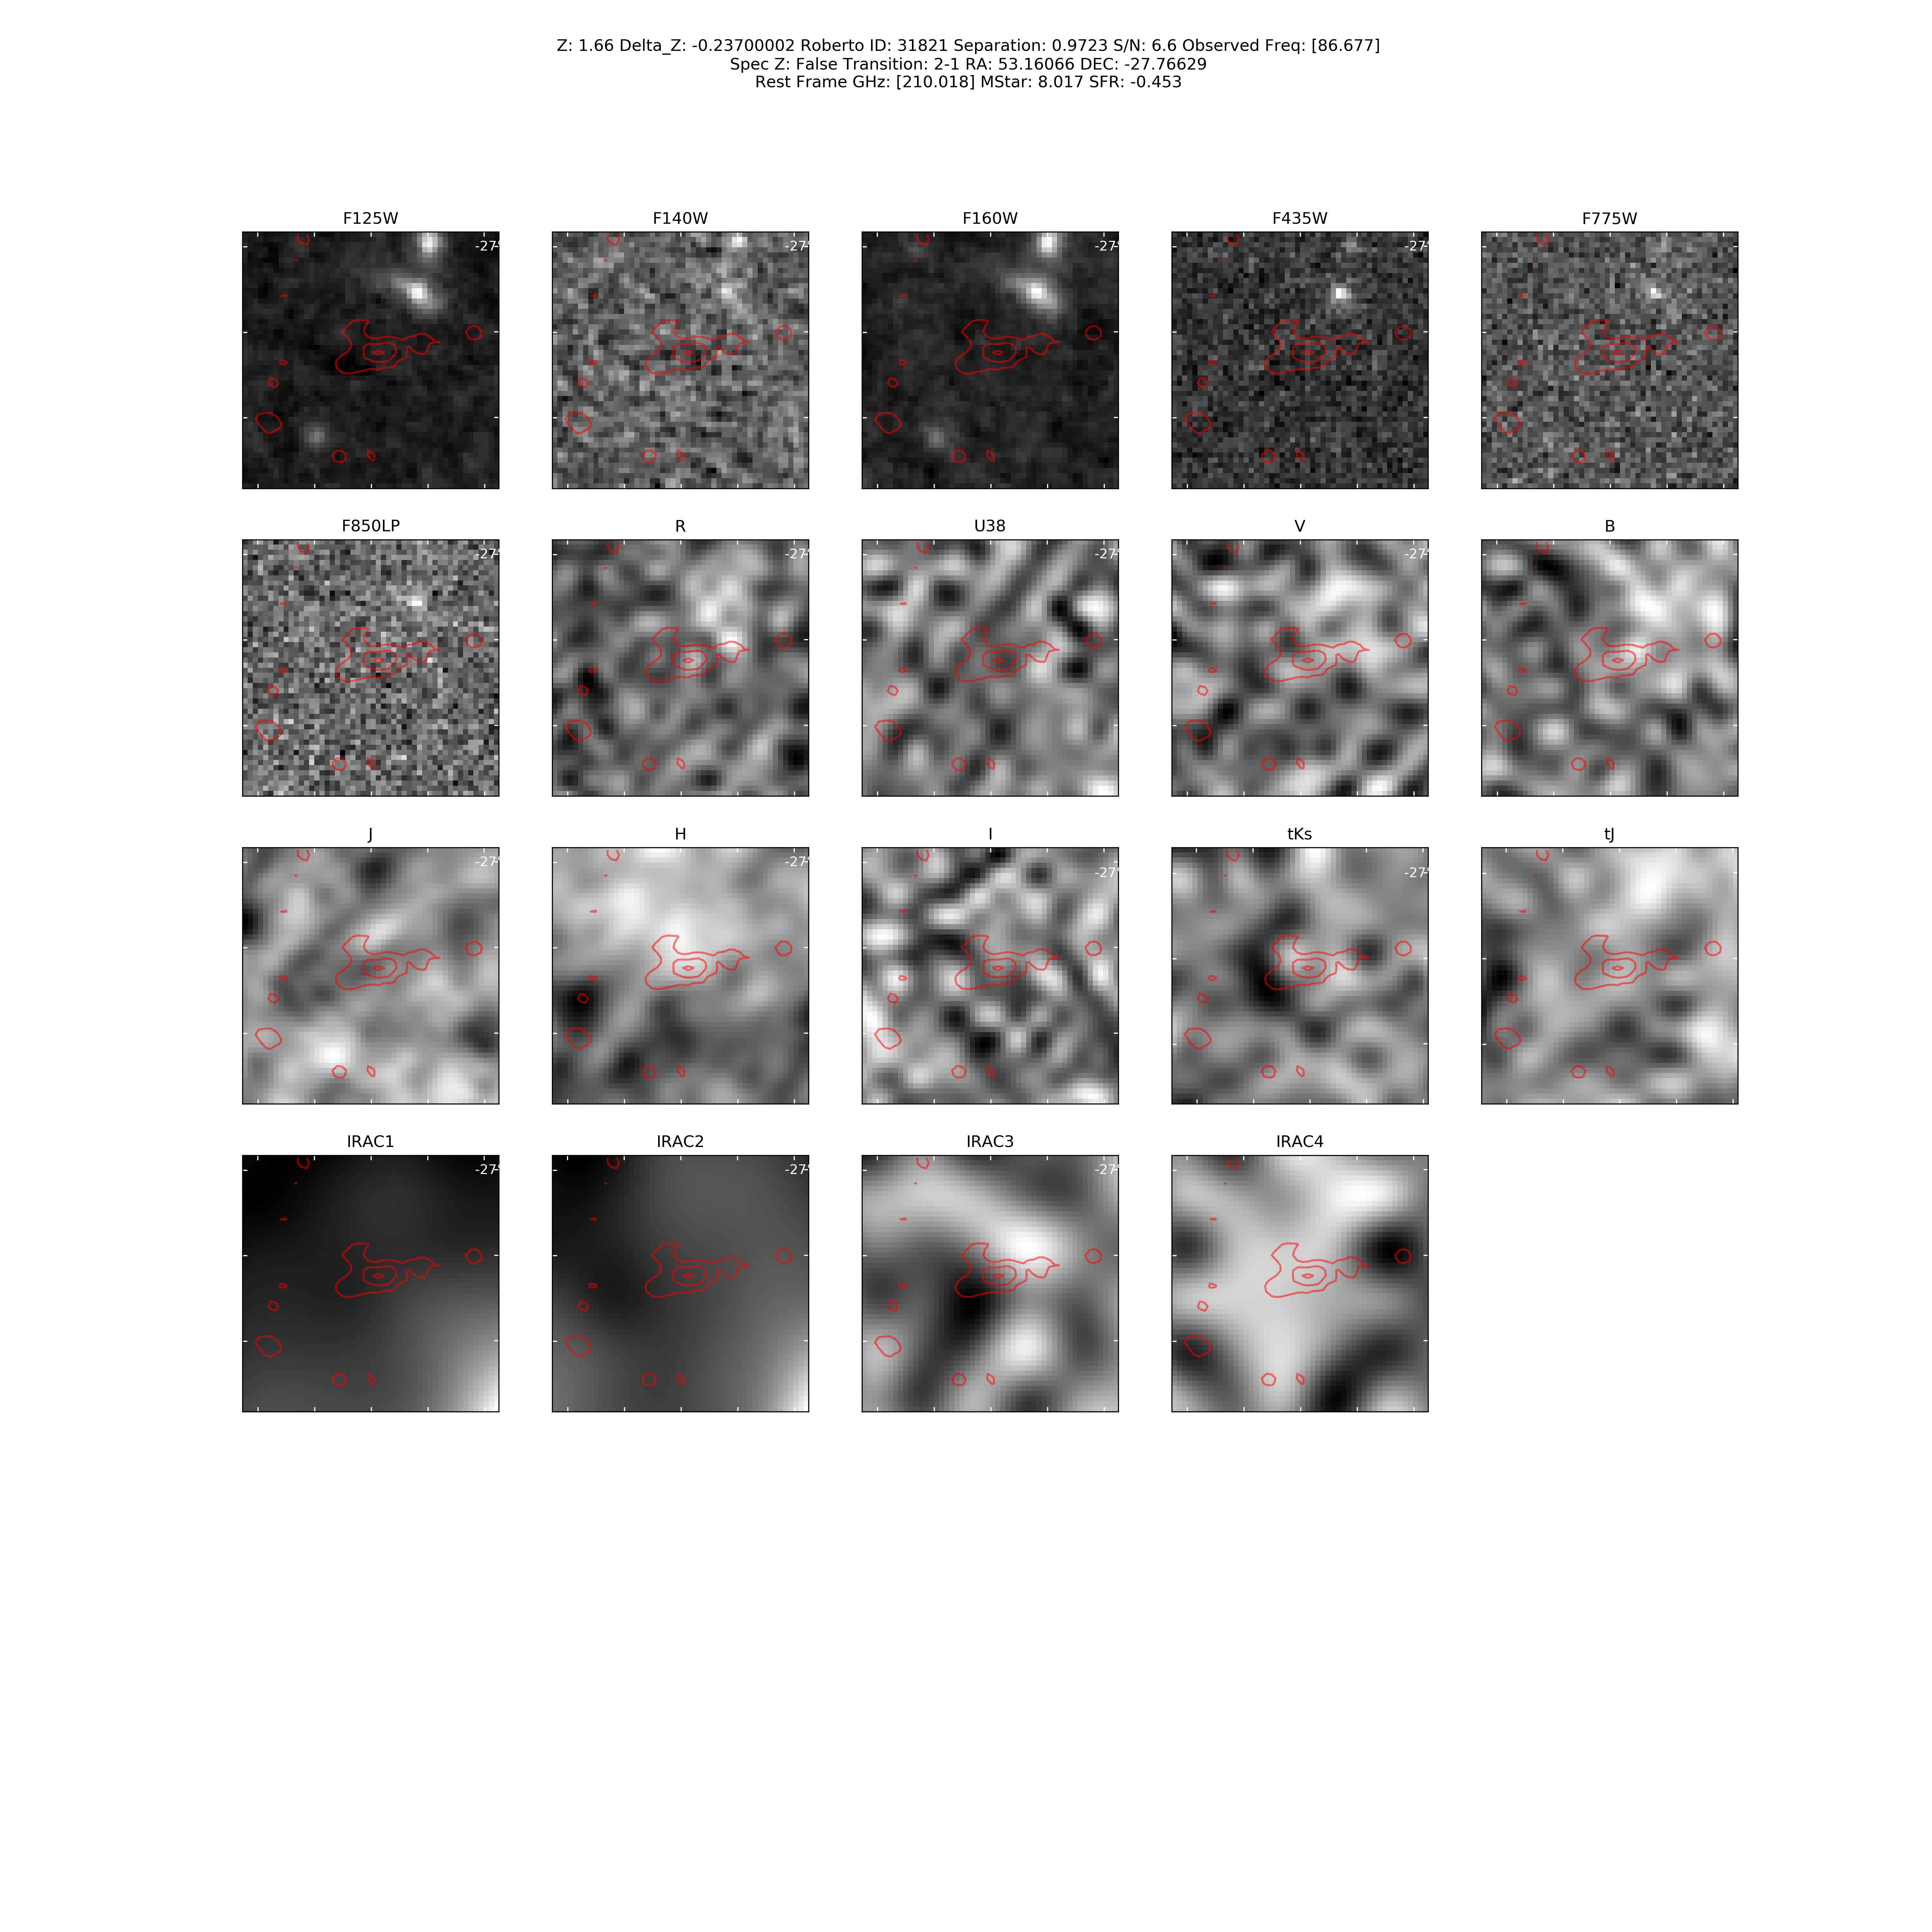
\includegraphics[width=160mm]{Matched/ASPECS_Cutout_12.png}
\caption{ID.13. Same contours and cutout size as for \ref{fig:Match_One}.}
\label{fig:Match_Three}
\end{figure}

\begin{figure}[tbp]
\centering 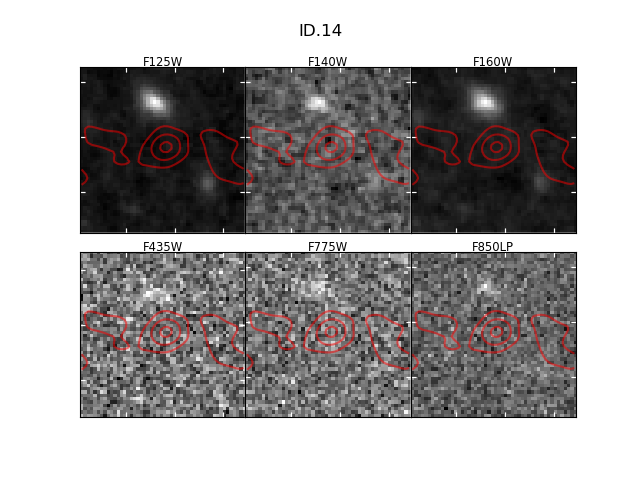
\includegraphics[width=160mm]{Matched/ASPECS_Cutout_13.png}
\caption{ID.14. Same contours and cutout size as for \ref{fig:Match_One}.}
\label{fig:Match_Three}
\end{figure}

\begin{figure}[tbp]
\centering 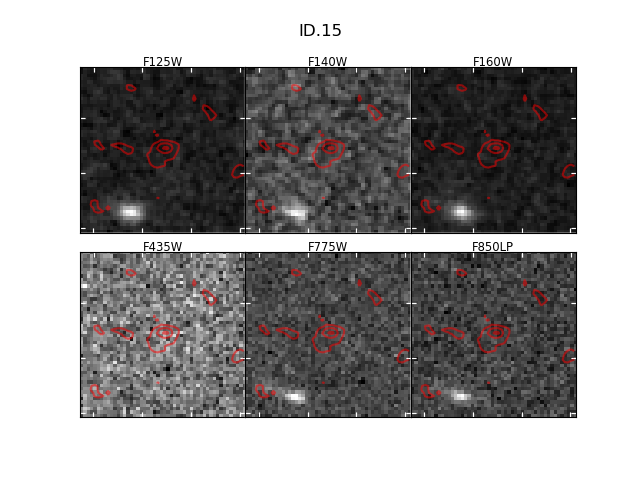
\includegraphics[width=160mm]{Matched/ASPECS_Cutout_14.png}
\caption{ID.15. Same contours and cutout size as for \ref{fig:Match_One}.}
\label{fig:Match_Three}
\end{figure}

\begin{figure}[tbp]
\centering 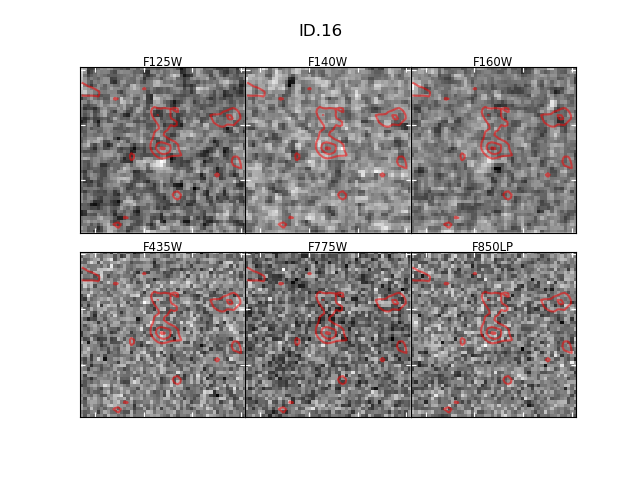
\includegraphics[width=160mm]{Matched/ASPECS_Cutout_15.png}
\caption{ID.16. Same contours and cutout size as for \ref{fig:Match_One}.}
\label{fig:Match_Three}
\end{figure}

\begin{figure}[tbp]
\centering 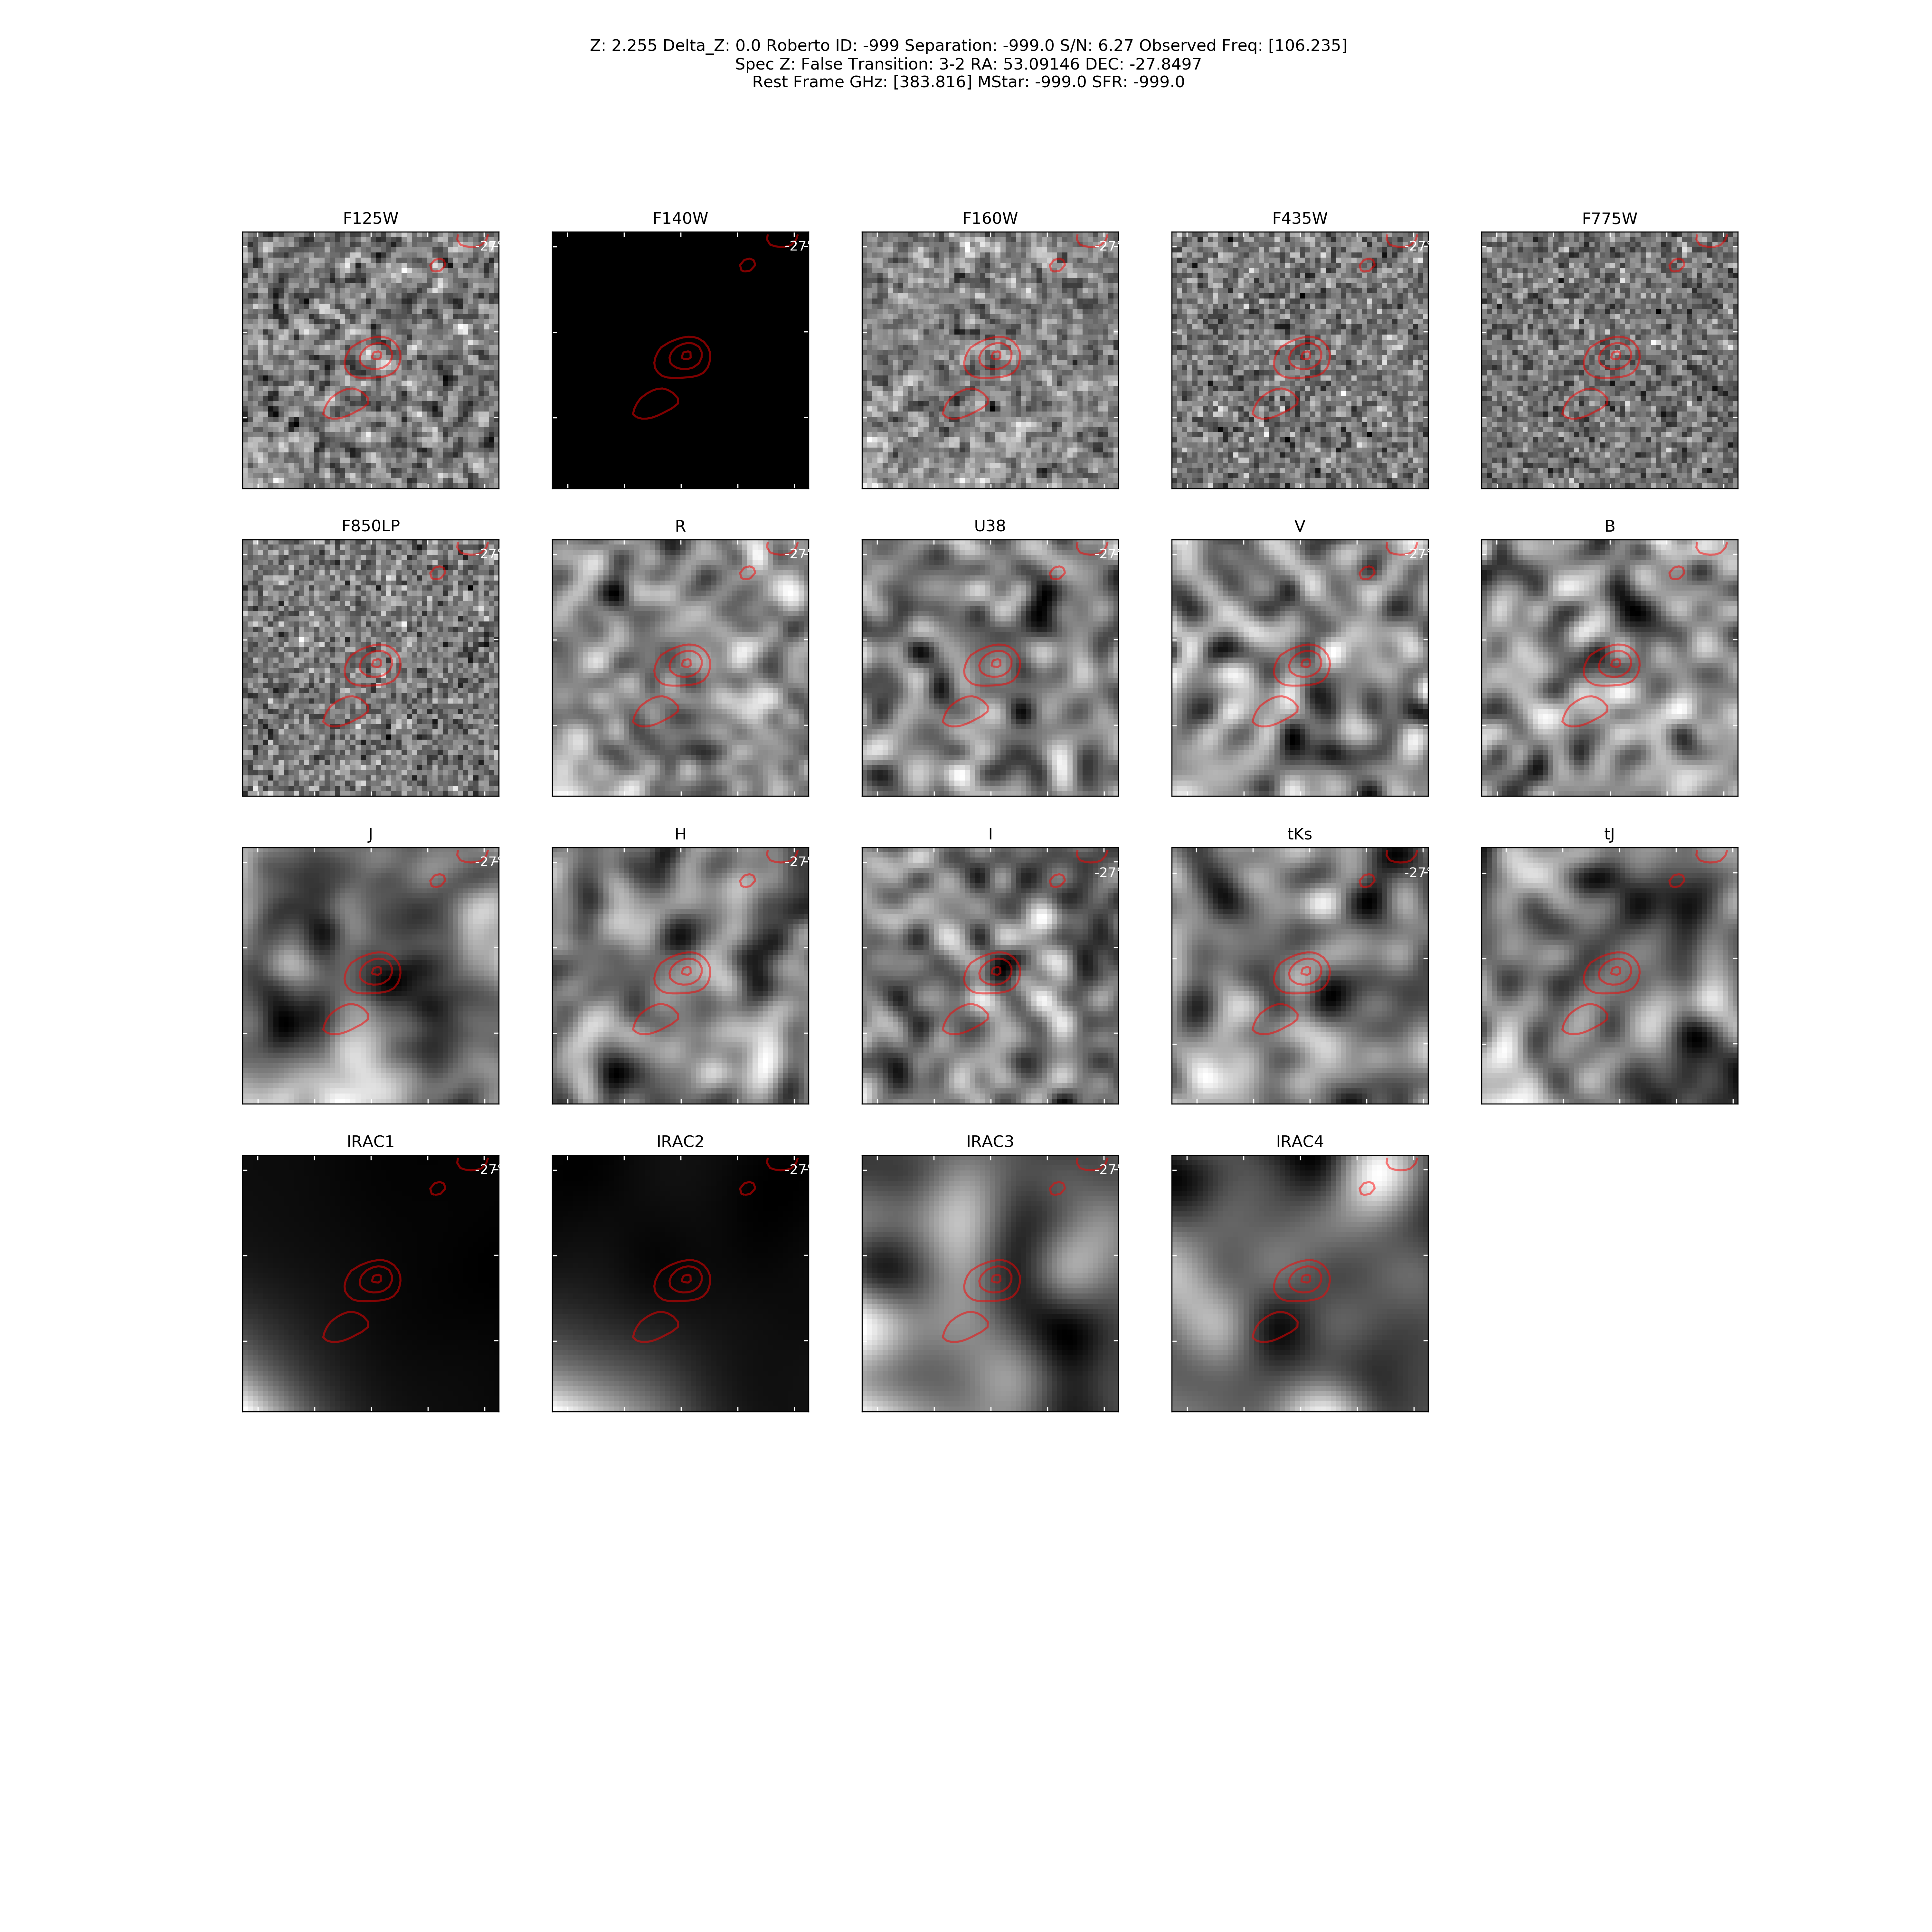
\includegraphics[width=160mm]{Matched/ASPECS_Cutout_16.png}
\caption{ID.17. Same contours and cutout size as for \ref{fig:Match_One}.}
\label{fig:Match_Three}
\end{figure}

\begin{figure}[tbp]
\centering 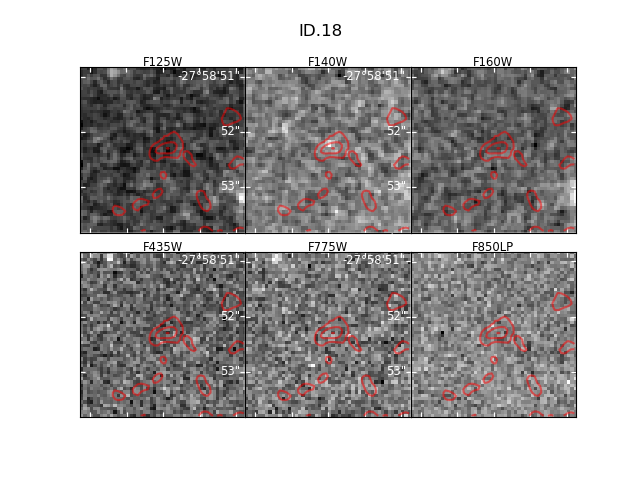
\includegraphics[width=160mm]{Matched/ASPECS_Cutout_17.png}
\caption{ID.18. Same contours and cutout size as for \ref{fig:Match_One}.}
\label{fig:Match_Three}
\end{figure}

\begin{figure}[tbp]
\centering 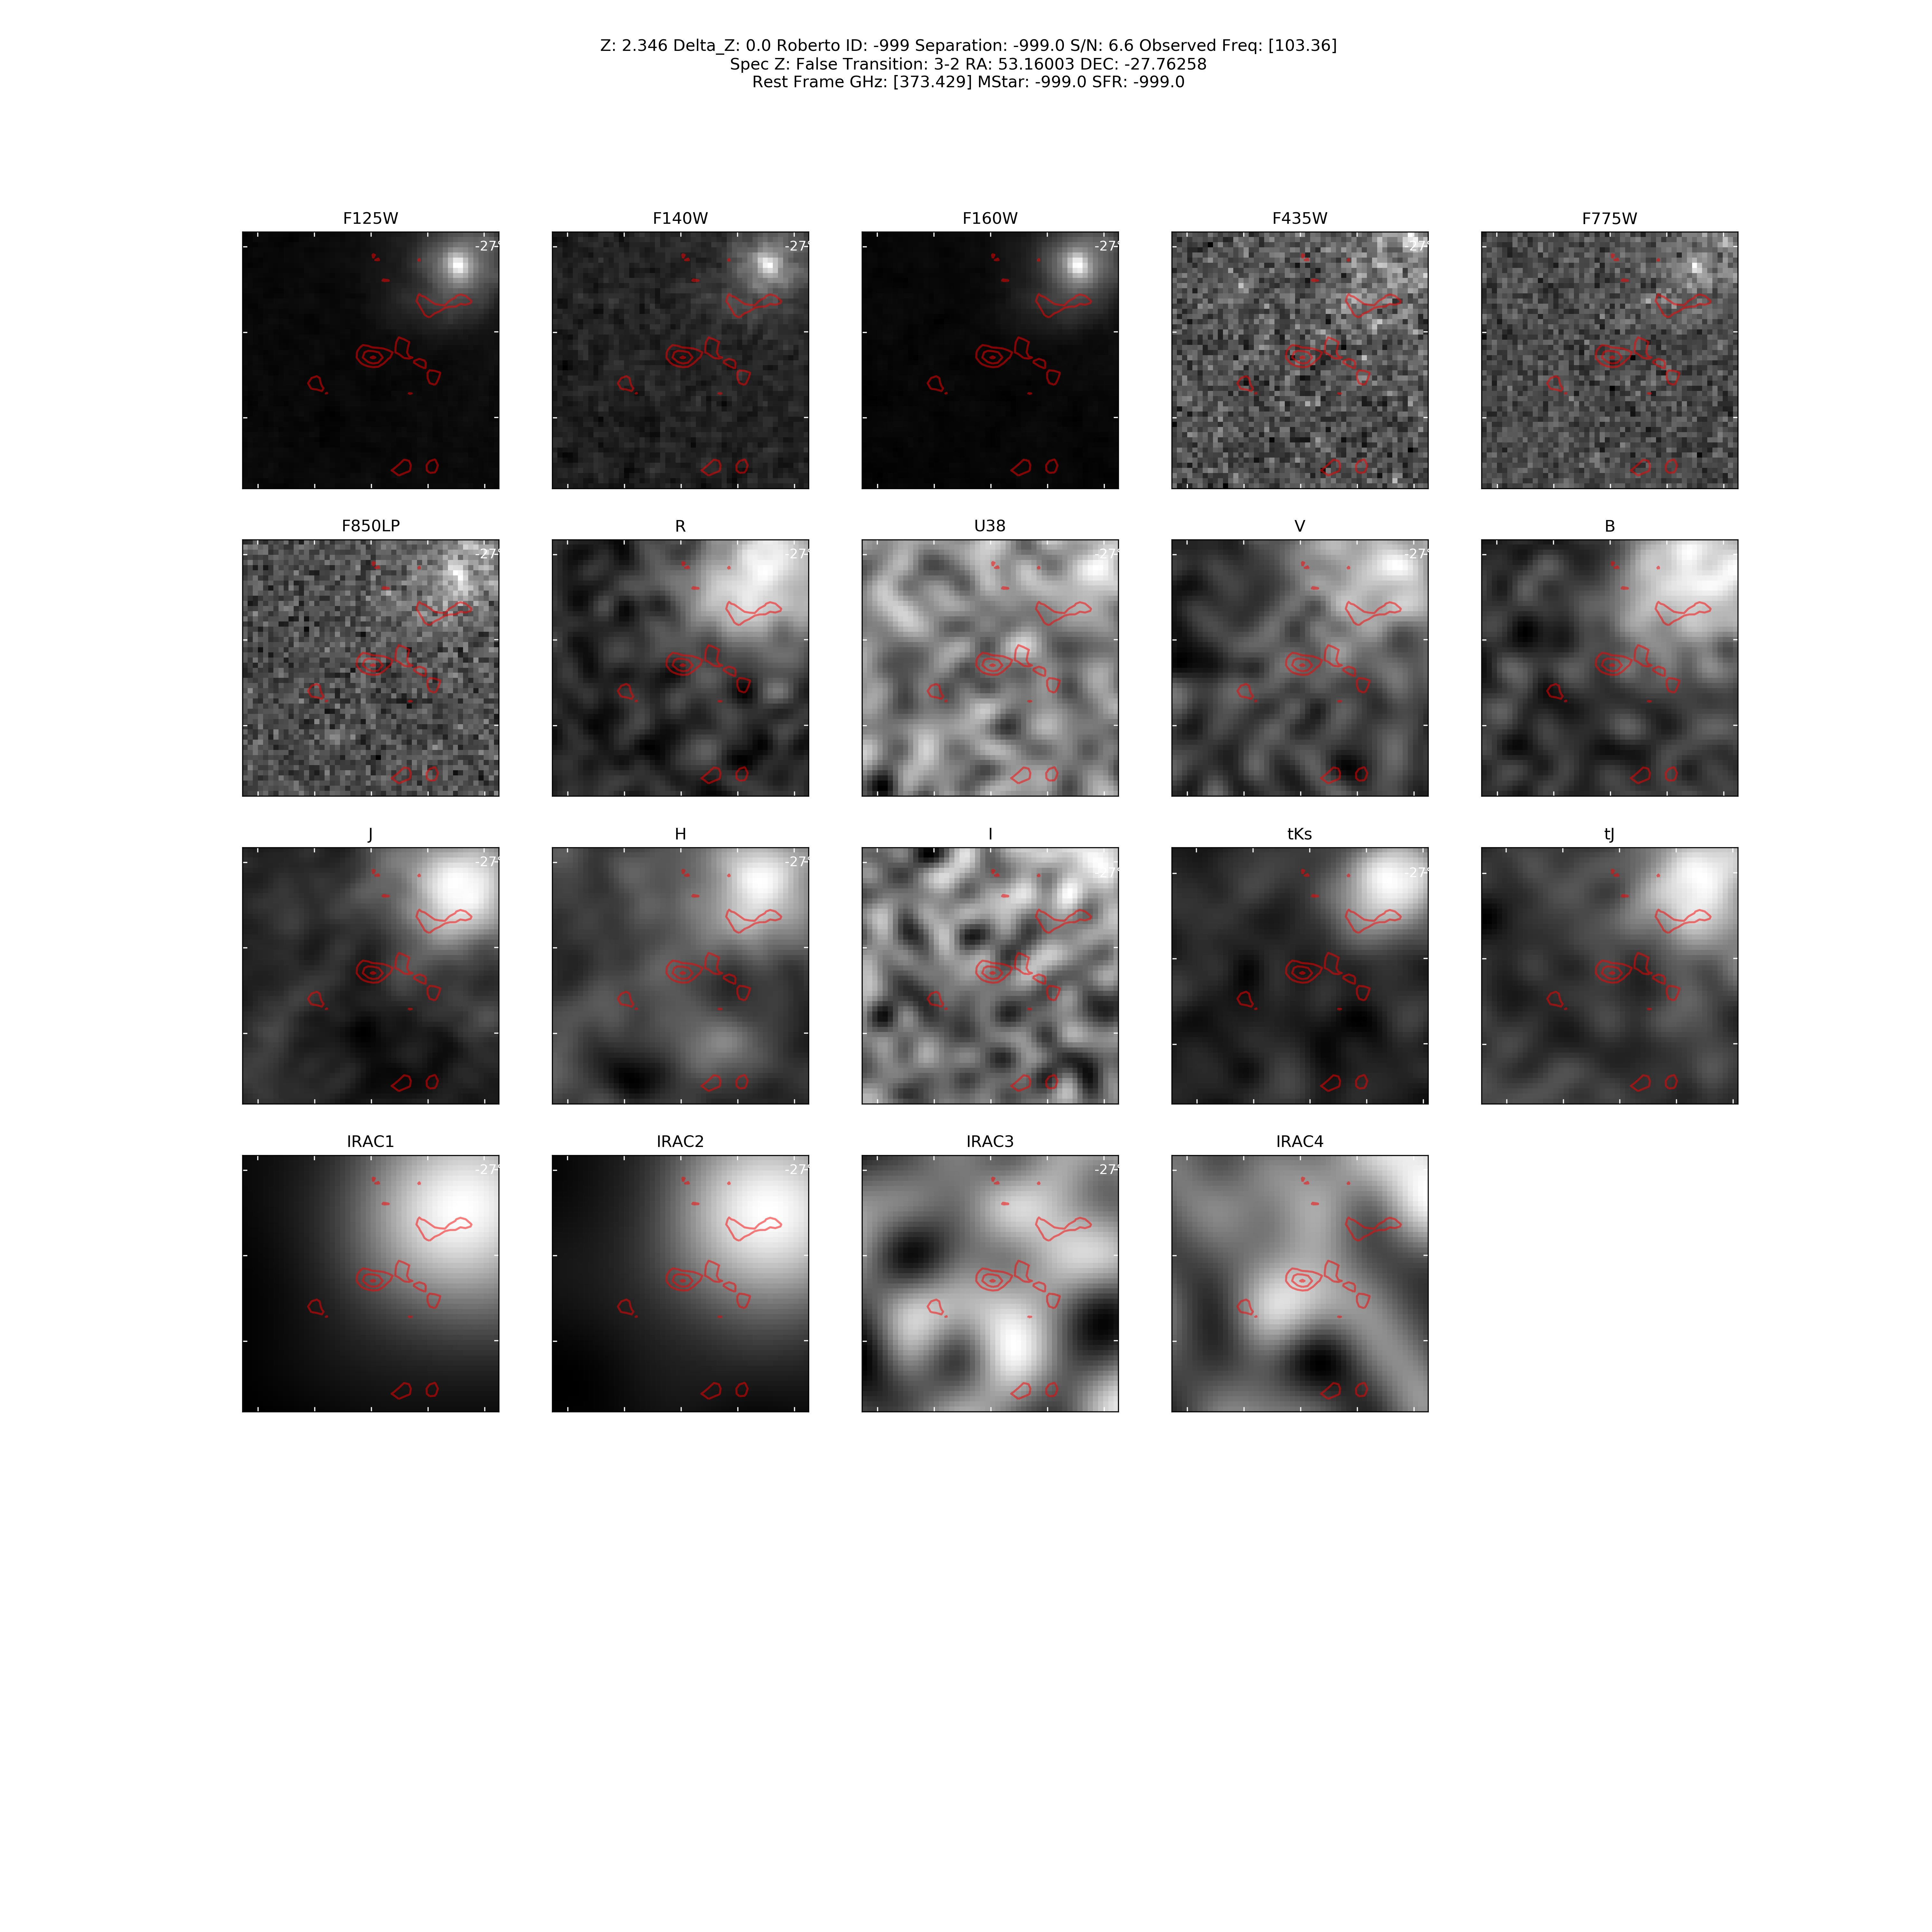
\includegraphics[width=160mm]{Matched/ASPECS_Cutout_18.png}
\caption{ID.19. Same contours and cutout size as for \ref{fig:Match_One}.}
\label{fig:Match_Three}
\end{figure}

\begin{figure}[tbp]
\centering 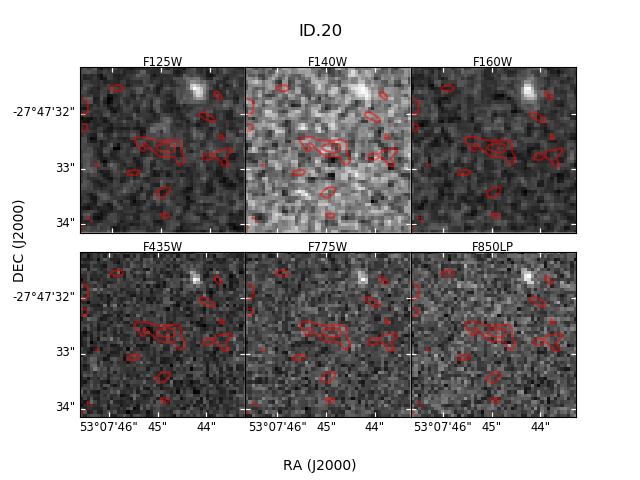
\includegraphics[width=160mm]{Matched/ASPECS_Cutout_19.png}
\caption{ID.20. Same contours and cutout size as for \ref{fig:Match_One}.}
\label{fig:Match_Three}
\end{figure}

\begin{figure}[tbp]
\centering 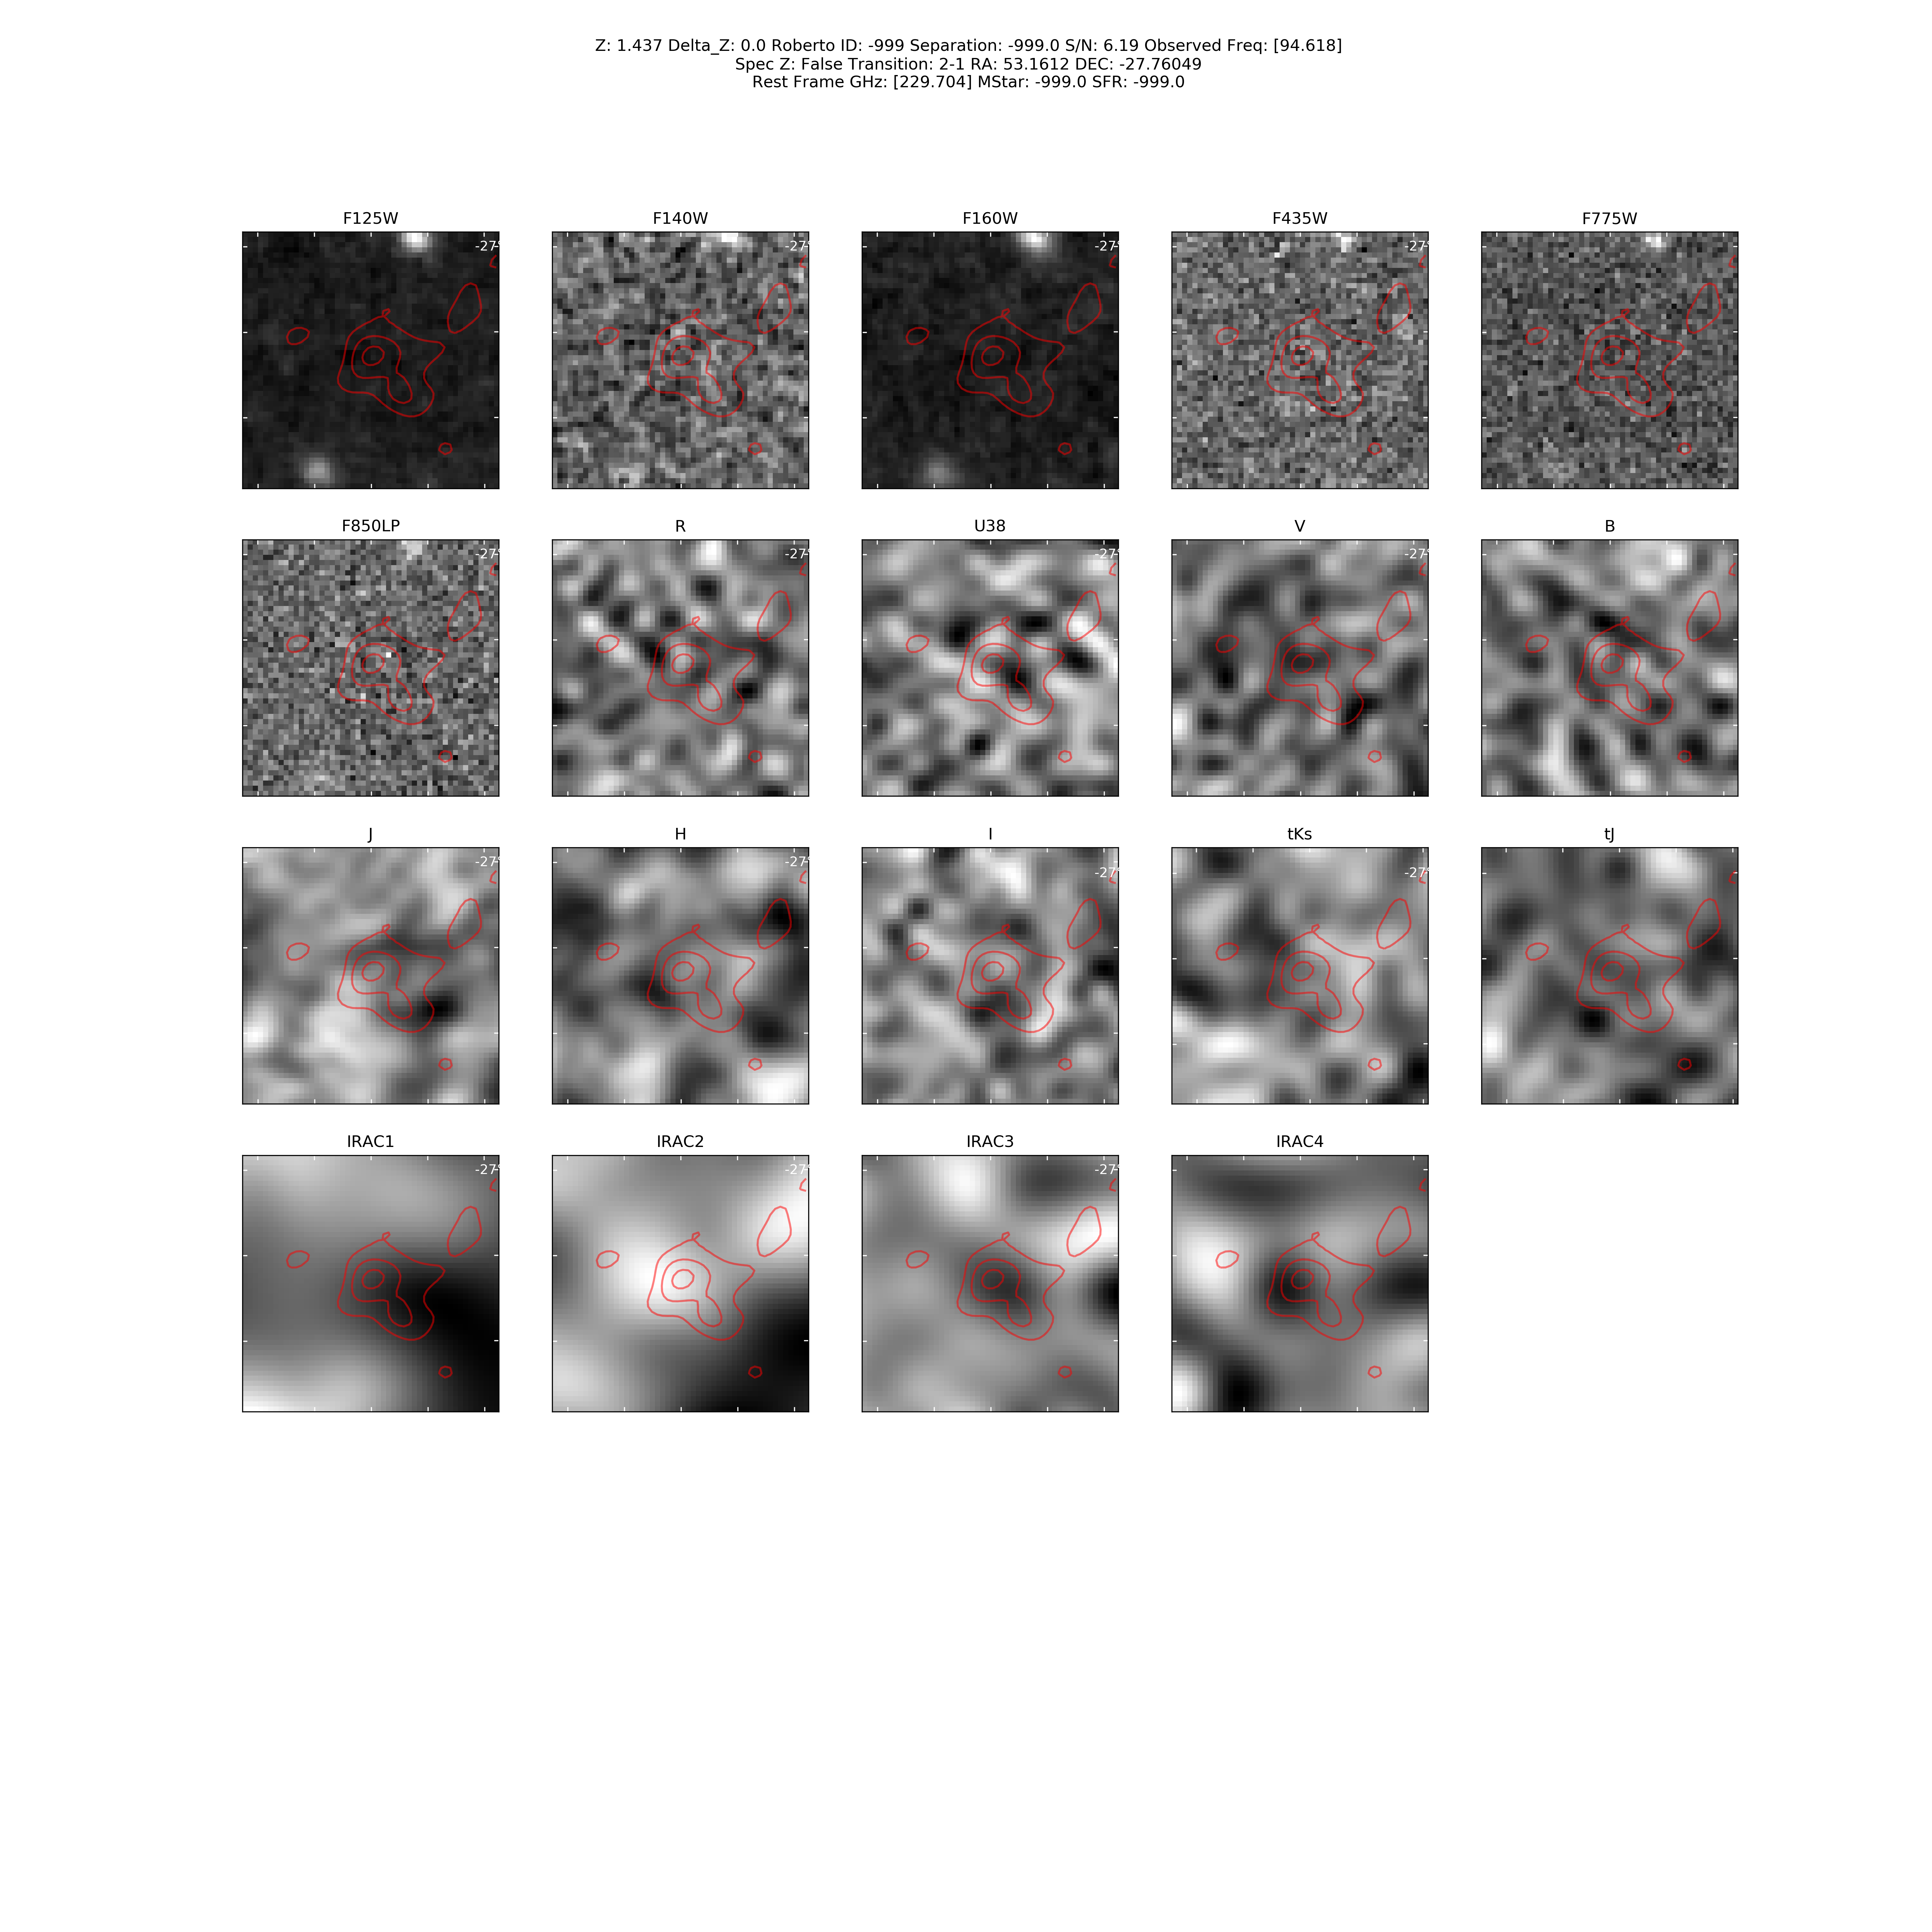
\includegraphics[width=160mm]{Matched/ASPECS_Cutout_20.png}
\caption{ID.21. Same contours and cutout size as for \ref{fig:Match_One}.}
\label{fig:Match_Three}
\end{figure}

\begin{figure}[tbp]
\centering 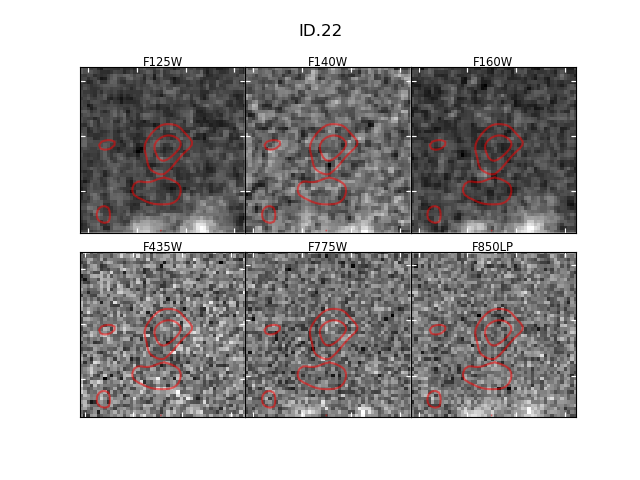
\includegraphics[width=160mm]{Matched/ASPECS_Cutout_21.png}
\caption{ID.22. Same contours and cutout size as for \ref{fig:Match_One}.}
\label{fig:Match_Three}
\end{figure}

\begin{figure}[tbp]
\centering 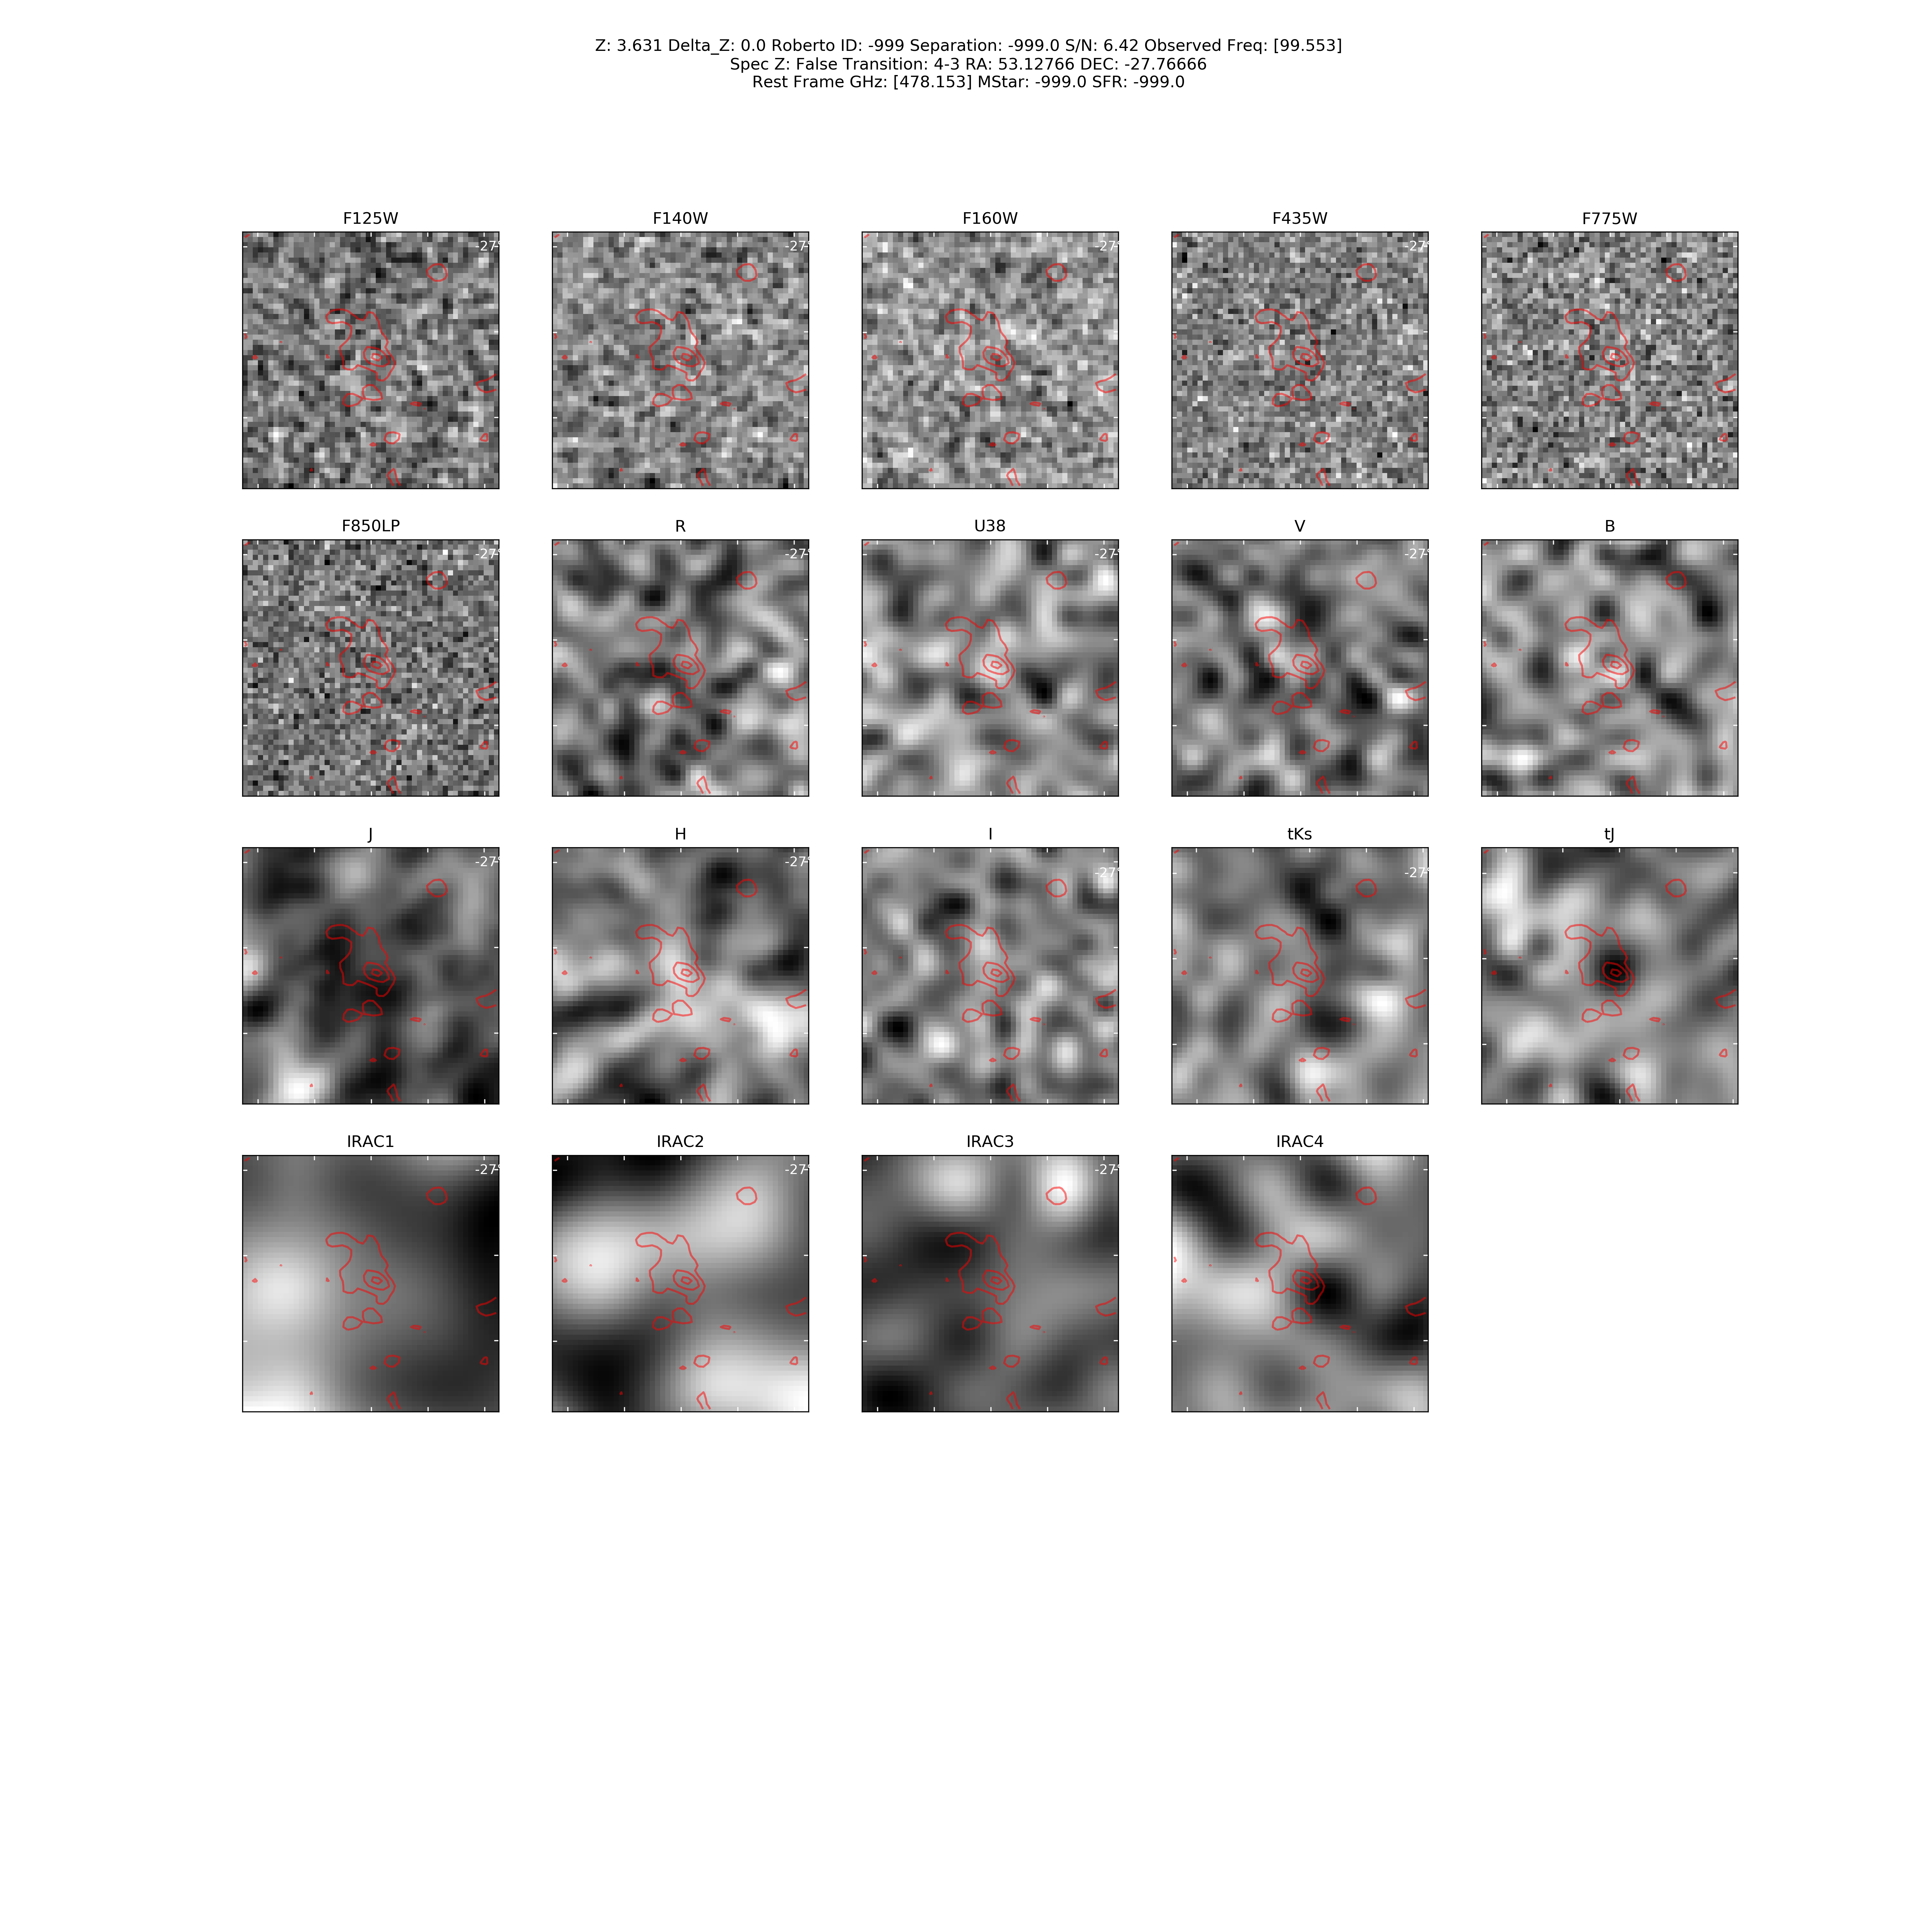
\includegraphics[width=160mm]{Matched/ASPECS_Cutout_22.png}
\caption{ID.23. Same contours and cutout size as for \ref{fig:Match_One}.}
\label{fig:Match_Three}
\end{figure}

\begin{figure}[tbp]
\centering 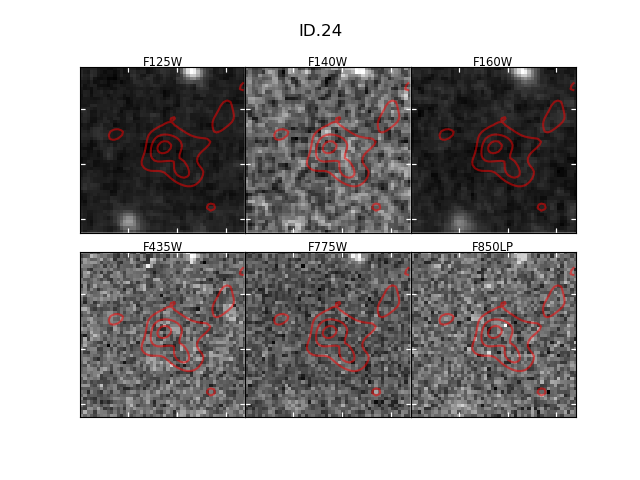
\includegraphics[width=160mm]{Matched/ASPECS_Cutout_23.png}
\caption{ID.24. Same contours and cutout size as for \ref{fig:Match_One}.}
\label{fig:Match_Three}
\end{figure}

\begin{figure}[tbp]
\centering 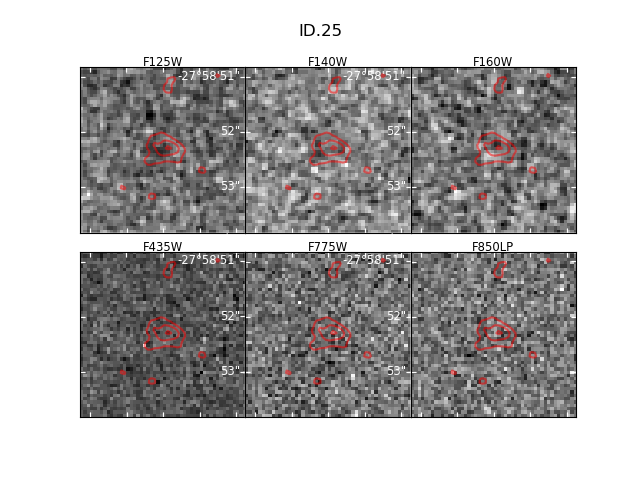
\includegraphics[width=160mm]{Matched/ASPECS_Cutout_24.png}
\caption{ID.25. Same contours and cutout size as for \ref{fig:Match_One}.}
\label{fig:Match_Three}
\end{figure}

\begin{figure}[tbp]
\centering 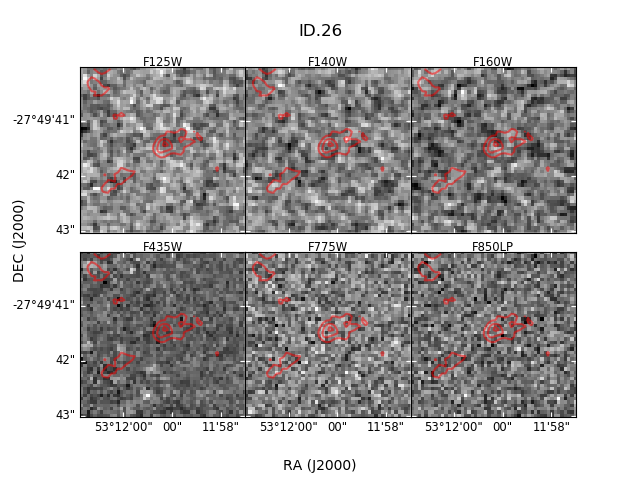
\includegraphics[width=160mm]{Matched/ASPECS_Cutout_25.png}
\caption{ID.26. Same contours and cutout size as for \ref{fig:Match_One}.}
\label{fig:Match_Three}
\end{figure}

\begin{figure}[tbp]
\centering 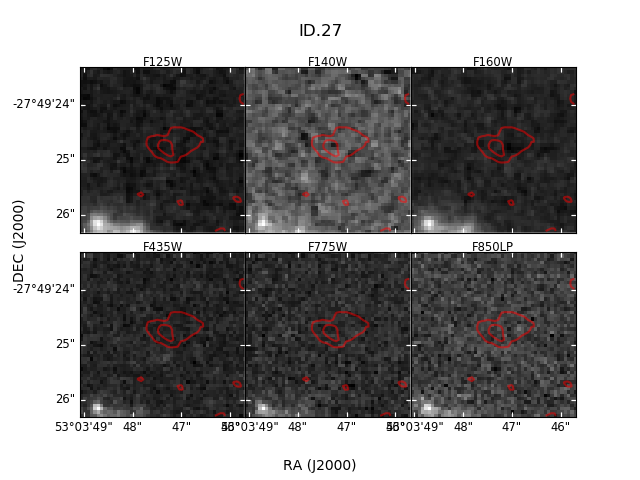
\includegraphics[width=160mm]{Matched/ASPECS_Cutout_26.png}
\caption{ID.27. Same contours and cutout size as for \ref{fig:Match_One}.}
\label{fig:Match_Three}
\end{figure}

\begin{figure}[tbp]
\centering 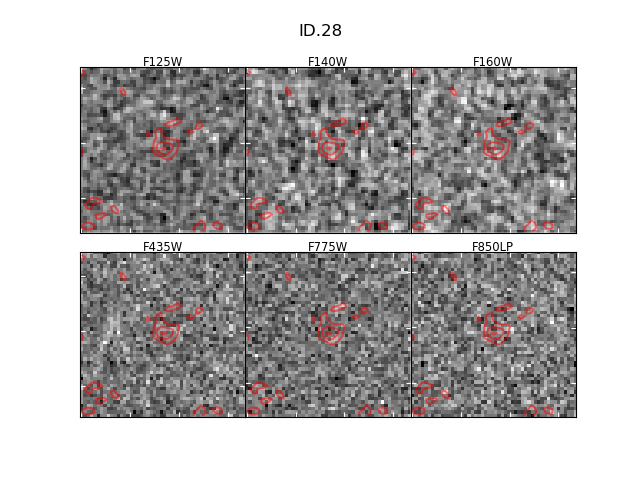
\includegraphics[width=160mm]{Matched/ASPECS_Cutout_27.png}
\caption{ID.28. Same contours and cutout size as for \ref{fig:Match_One}.}
\label{fig:Match_Three}
\end{figure}

\begin{figure}[tbp]
\centering 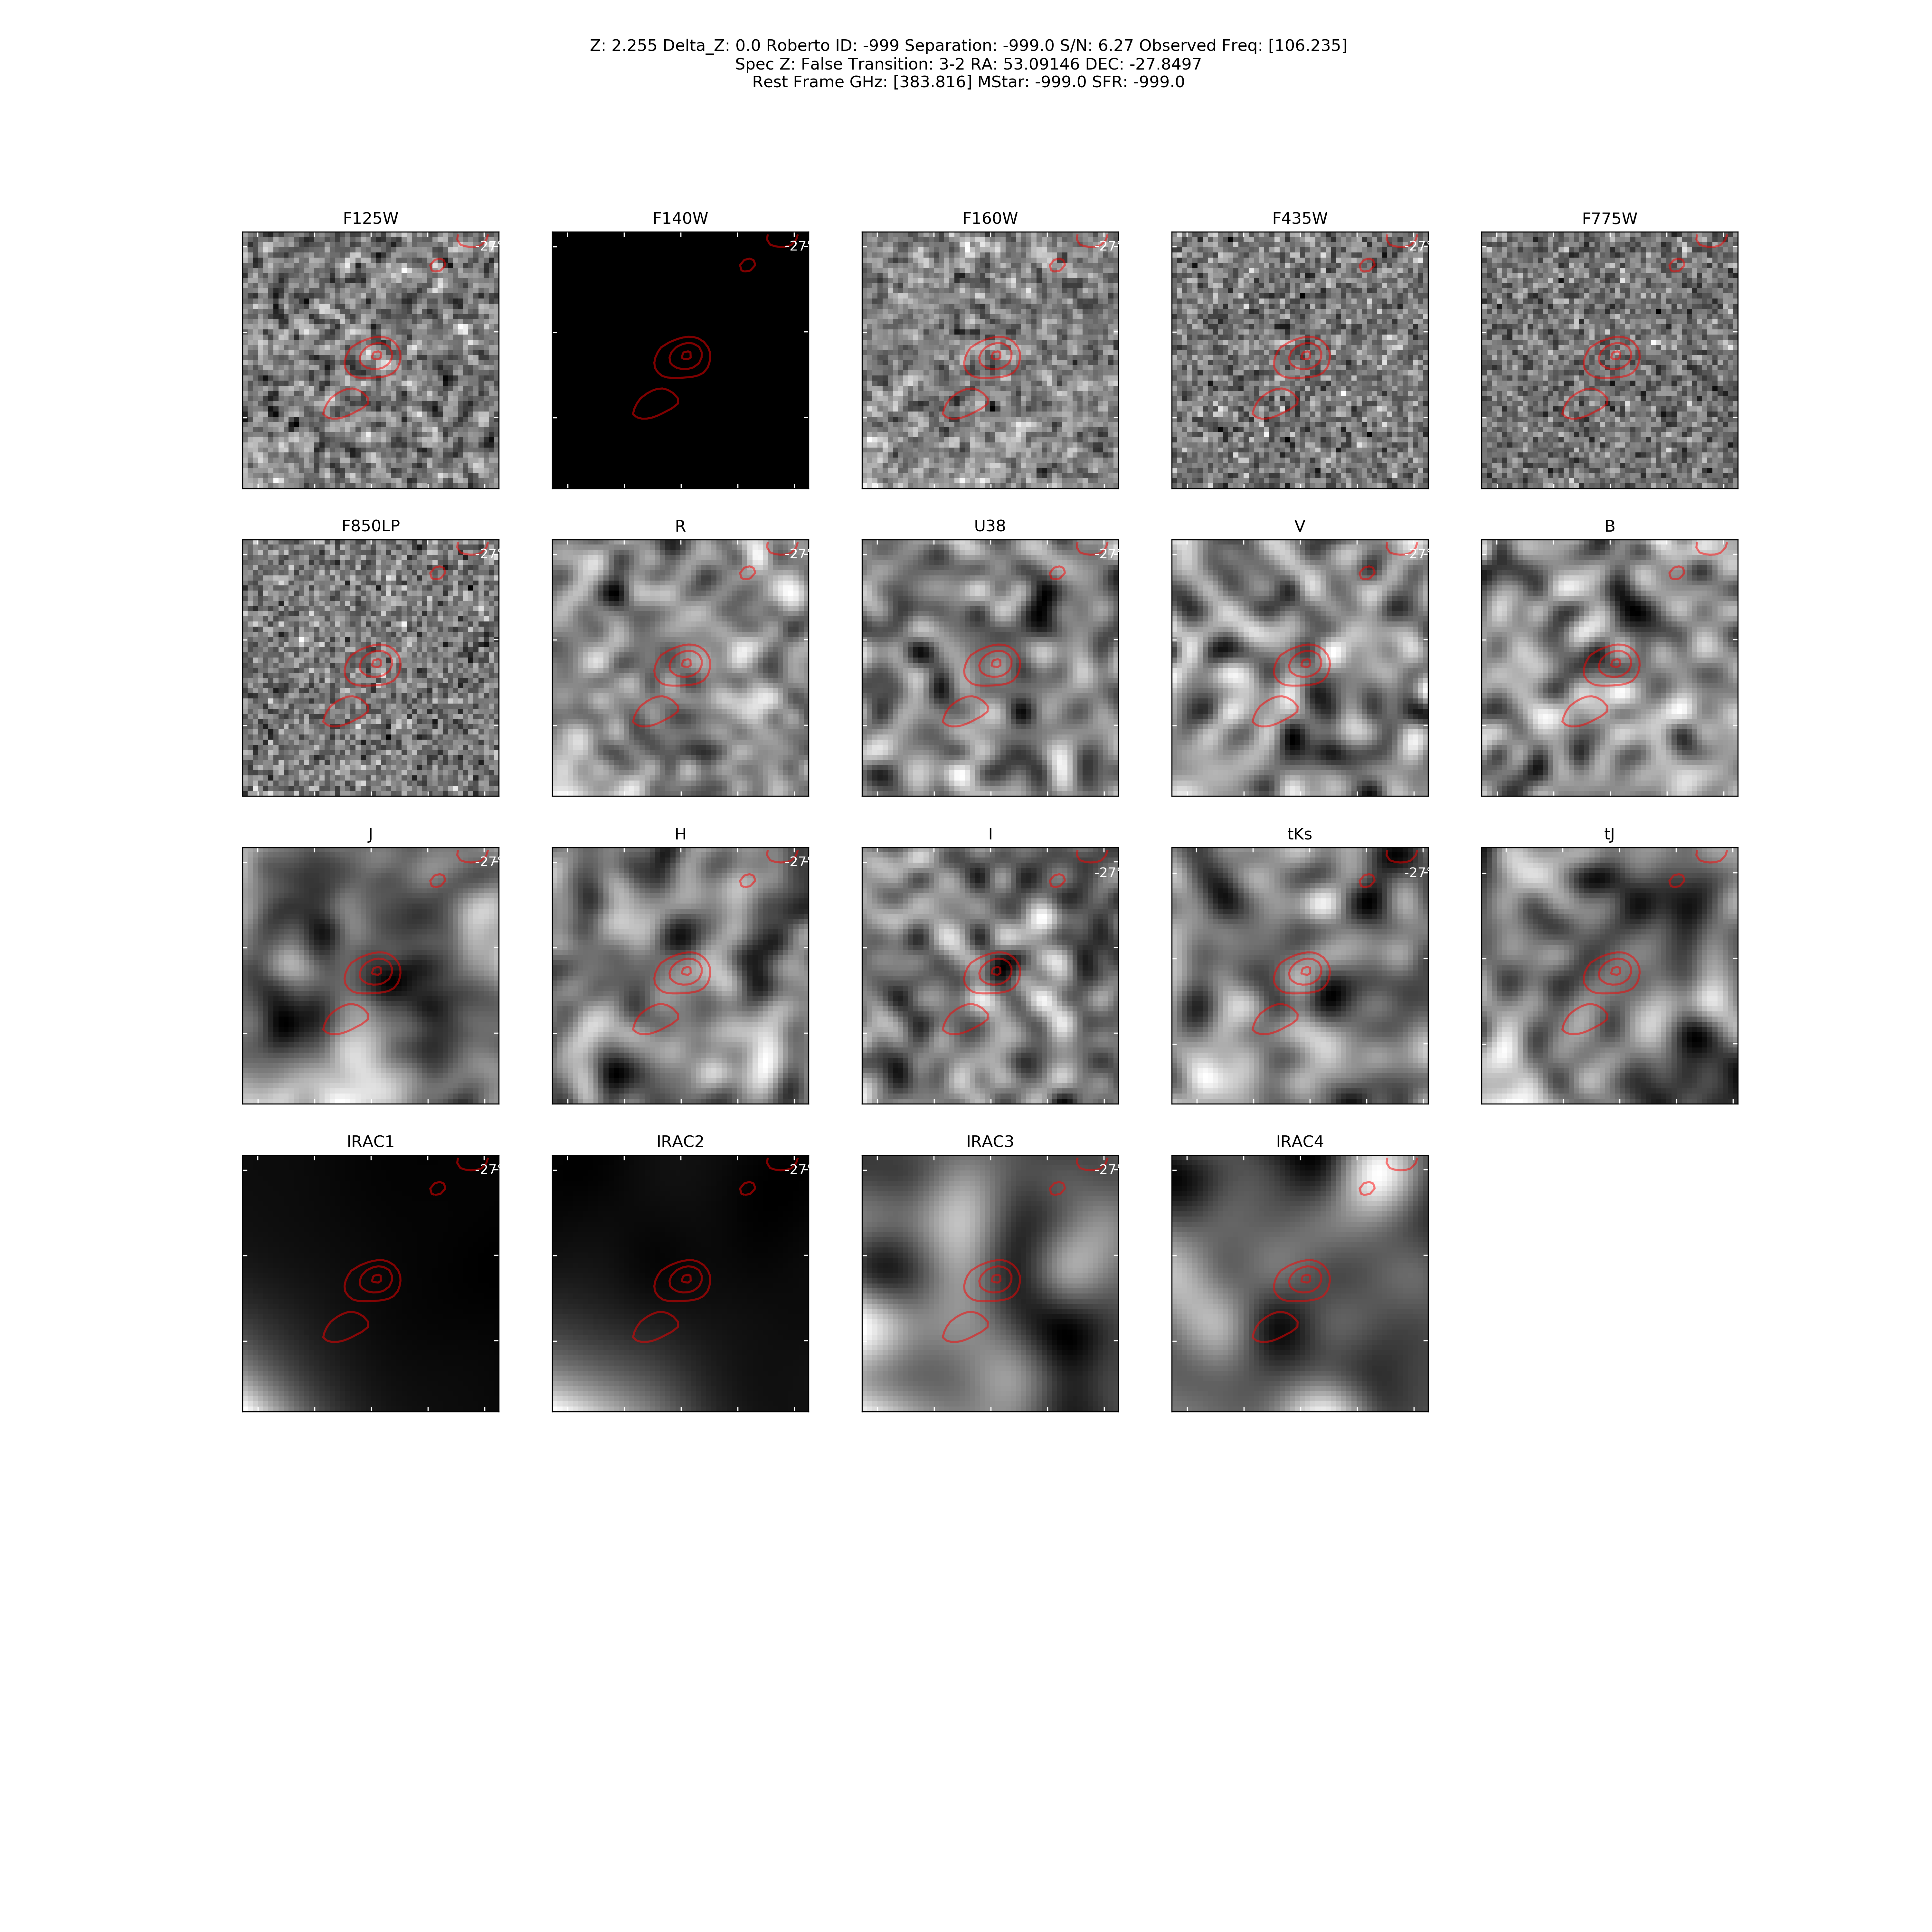
\includegraphics[width=160mm]{Matched/ASPECS_Cutout_28.png}
\caption{ID.29. Same contours and cutout size as for \ref{fig:Match_One}.}
\label{fig:Match_Three}
\end{figure}

\begin{figure}[tbp]
\centering 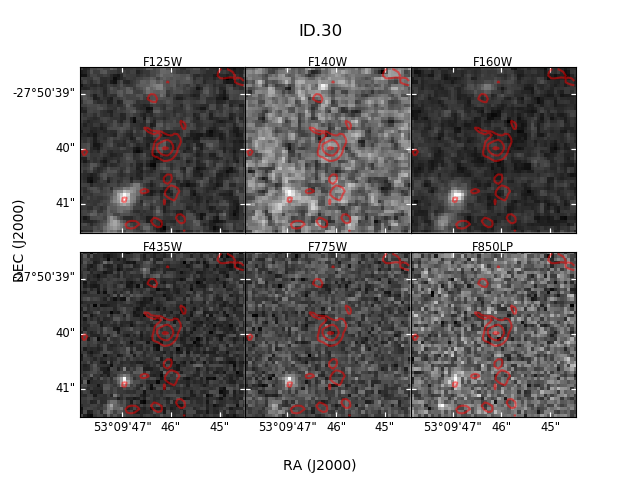
\includegraphics[width=160mm]{Matched/ASPECS_Cutout_29.png}
\caption{ID.30. Same contours and cutout size as for \ref{fig:Match_One}.}
\label{fig:Match_Three}
\end{figure}

\begin{figure}[tbp]
\centering 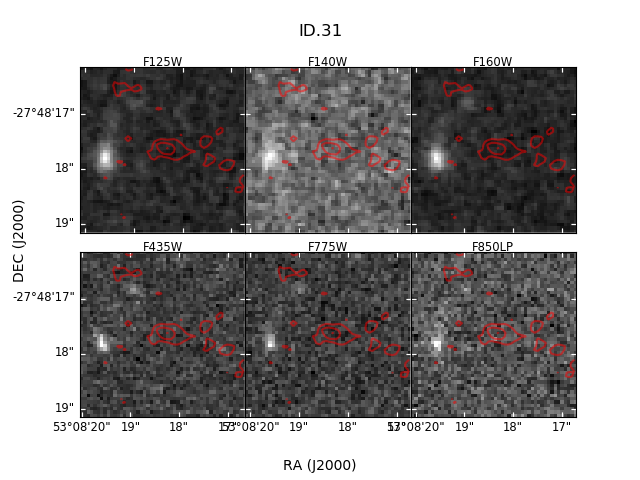
\includegraphics[width=160mm]{Matched/ASPECS_Cutout_30.png}
\caption{ID.31. Same contours and cutout size as for \ref{fig:Match_One}.}
\label{fig:Match_Three}
\end{figure}

\begin{figure}[tbp]
\centering 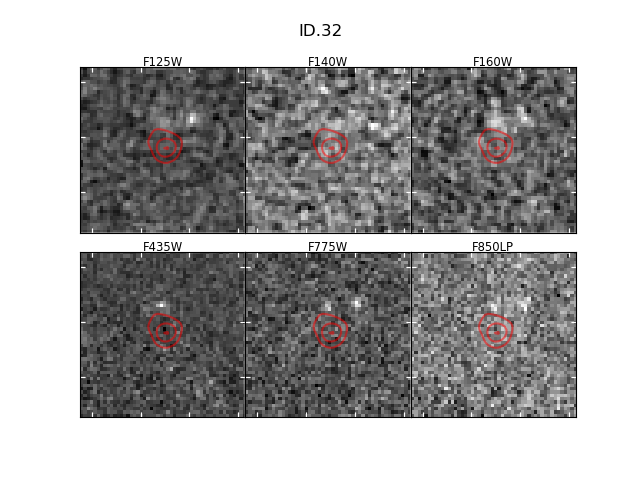
\includegraphics[width=160mm]{Matched/ASPECS_Cutout_31.png}
\caption{ID.32. Same contours and cutout size as for \ref{fig:Match_One}.}
\label{fig:Match_Three}
\end{figure}

\begin{figure}[tbp]
\centering 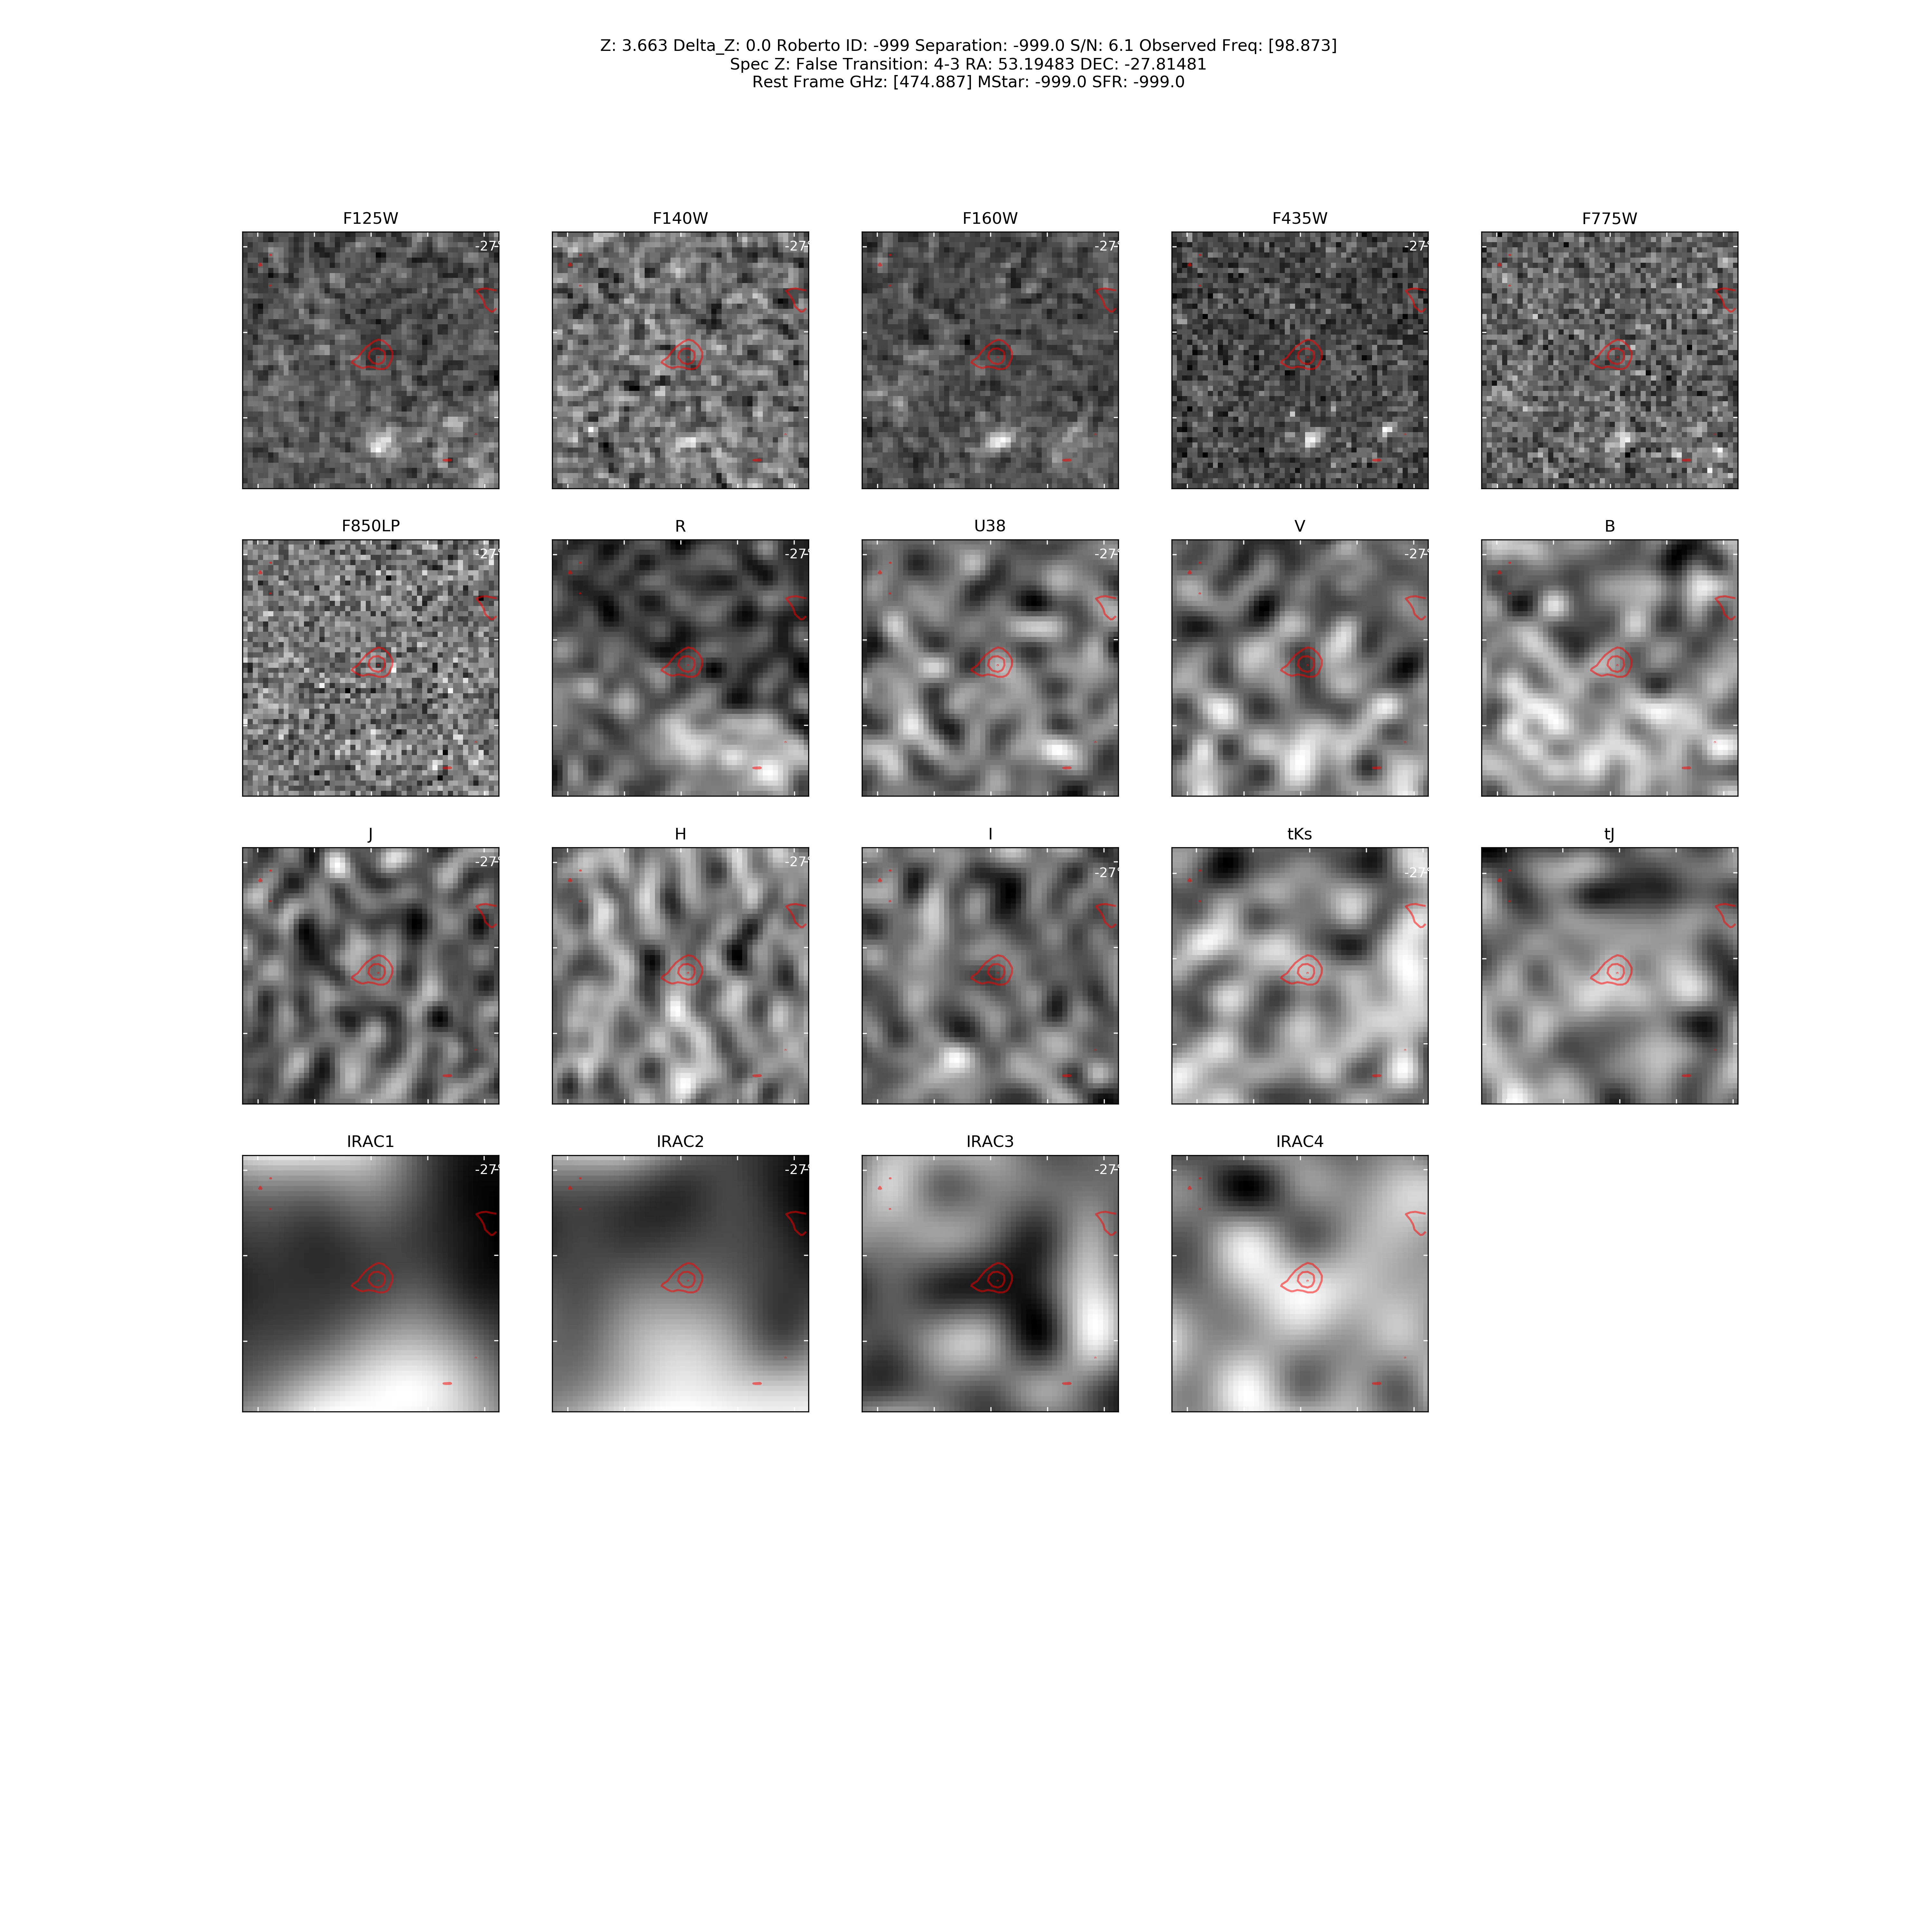
\includegraphics[width=160mm]{Matched/ASPECS_Cutout_32.png}
\caption{ID.33. Same contours and cutout size as for \ref{fig:Match_One}.}
\label{fig:Match_Three}
\end{figure}

\begin{figure}[tbp]
\centering 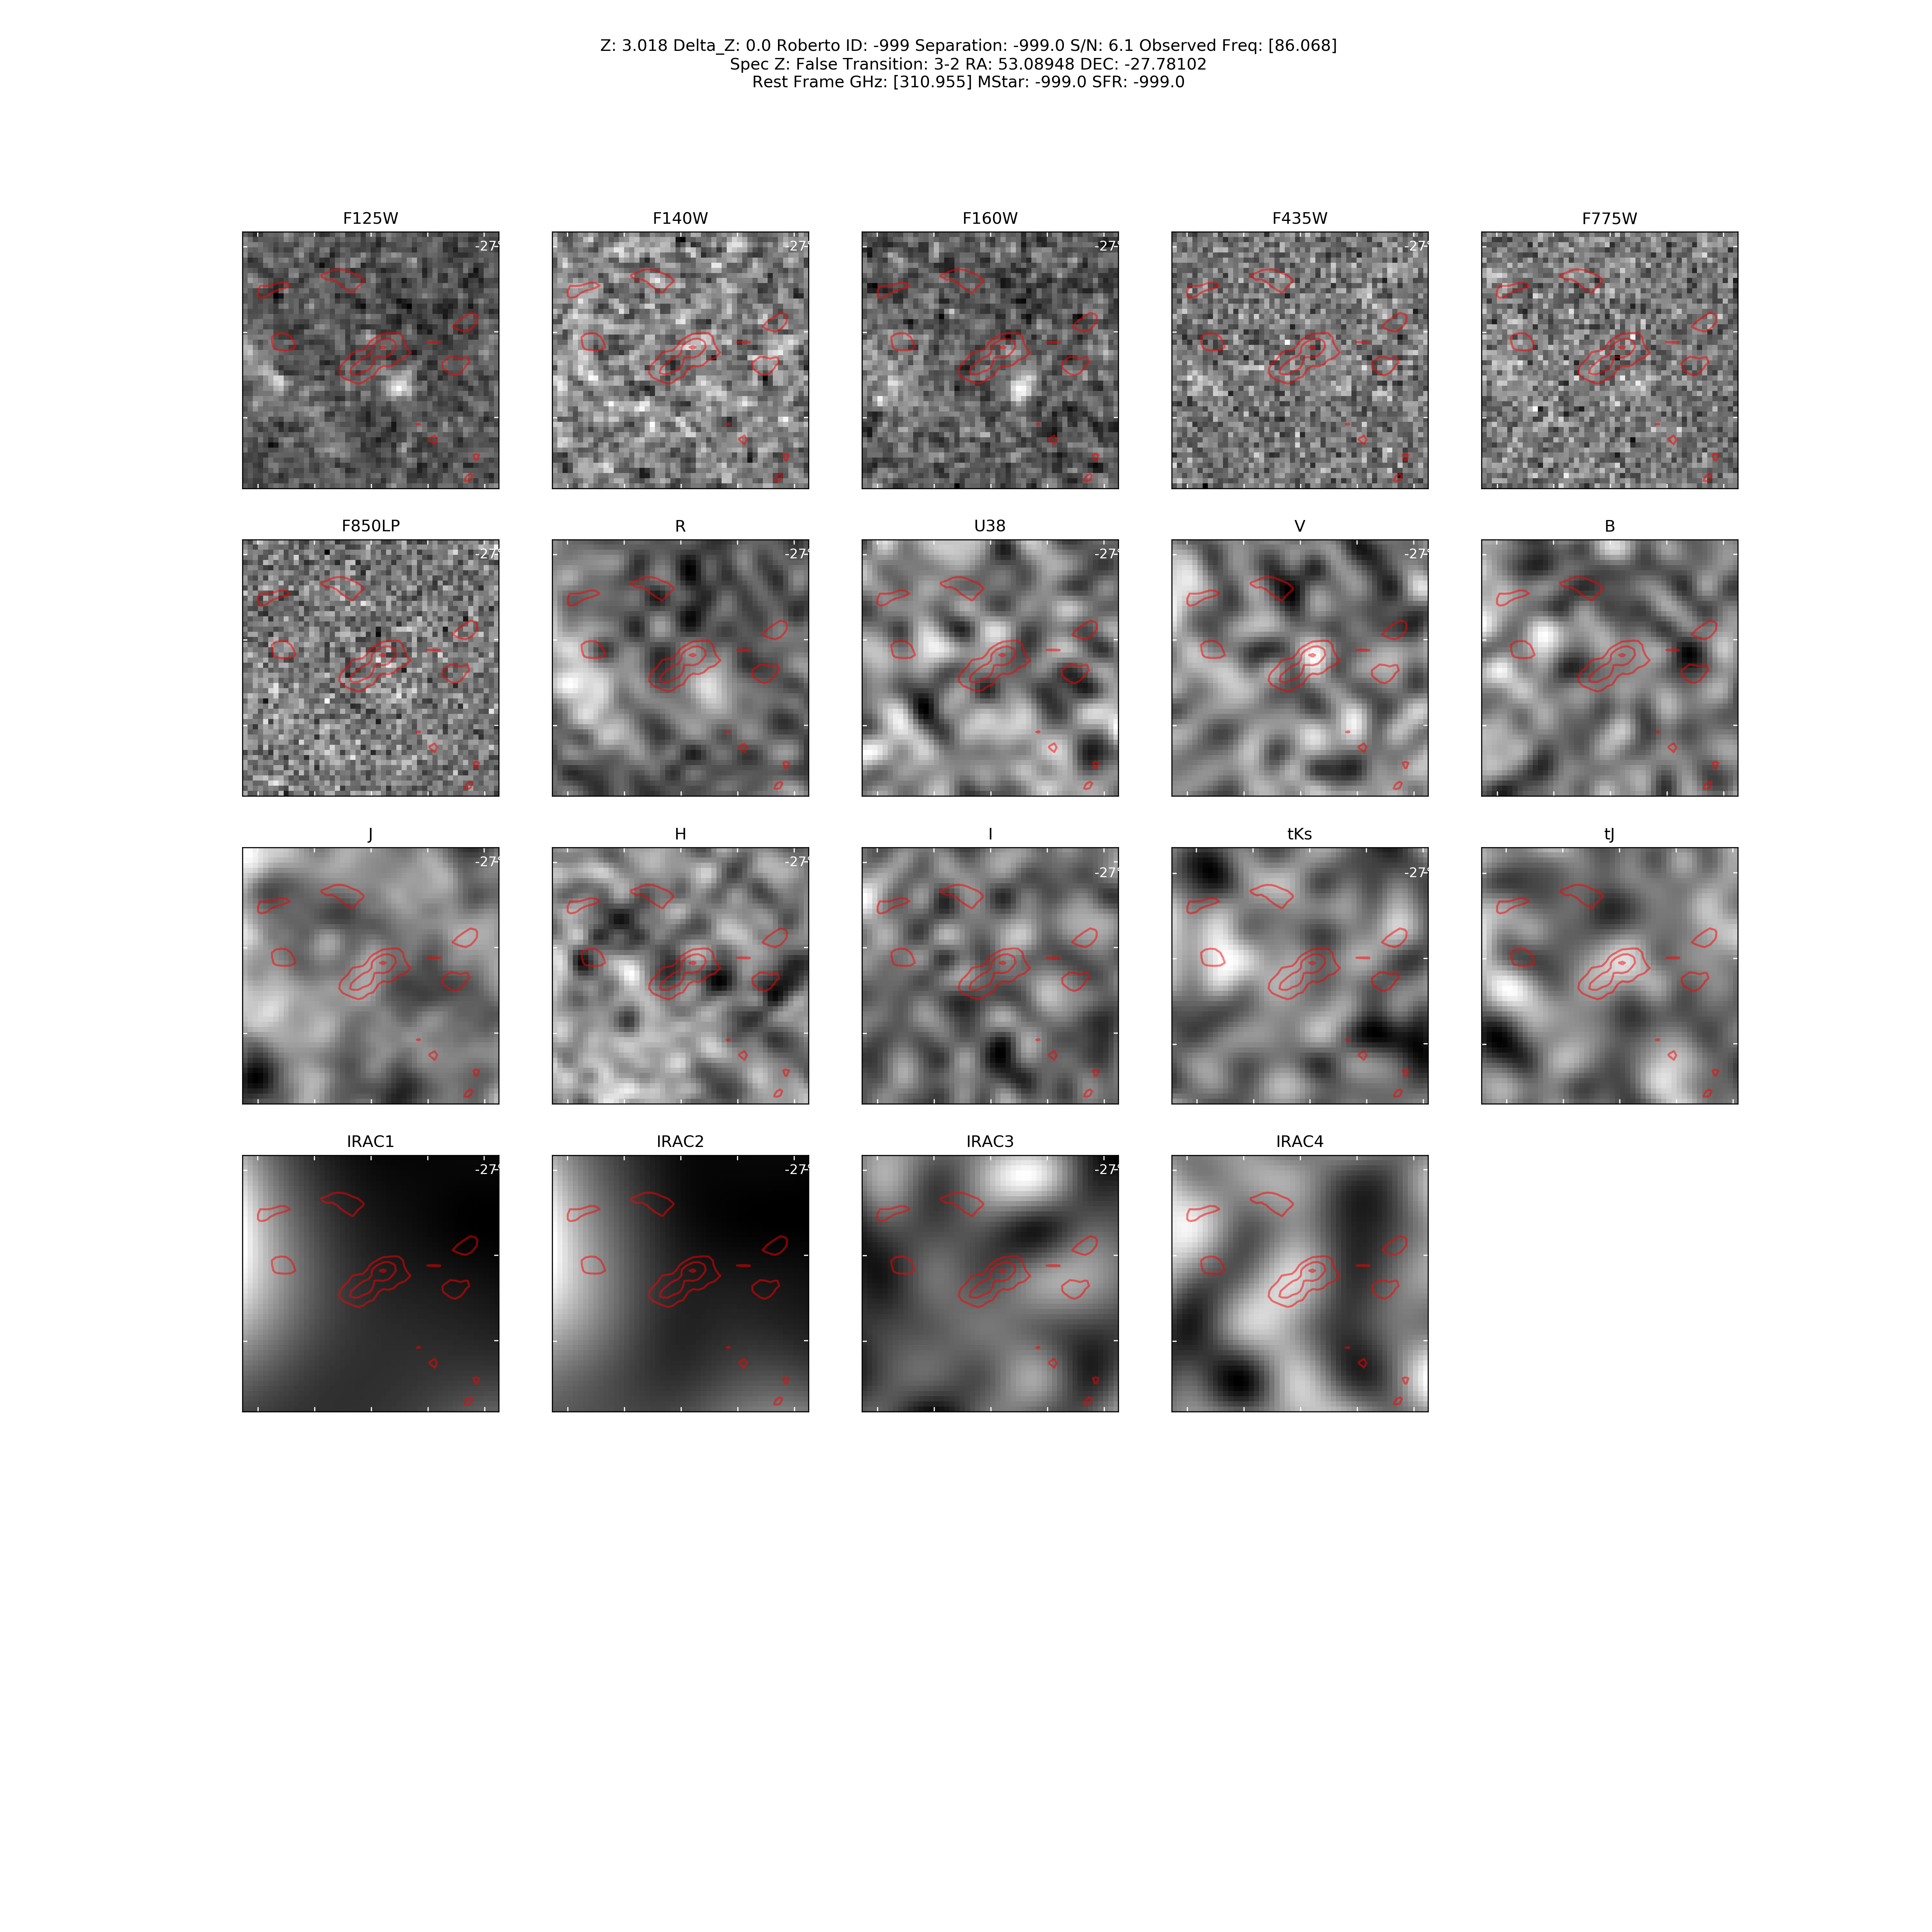
\includegraphics[width=160mm]{Matched/ASPECS_Cutout_33.png}
\caption{ID.34. Same contours and cutout size as for \ref{fig:Match_One}.}
\label{fig:Match_Three}
\end{figure}

\begin{figure}[tbp]
\centering 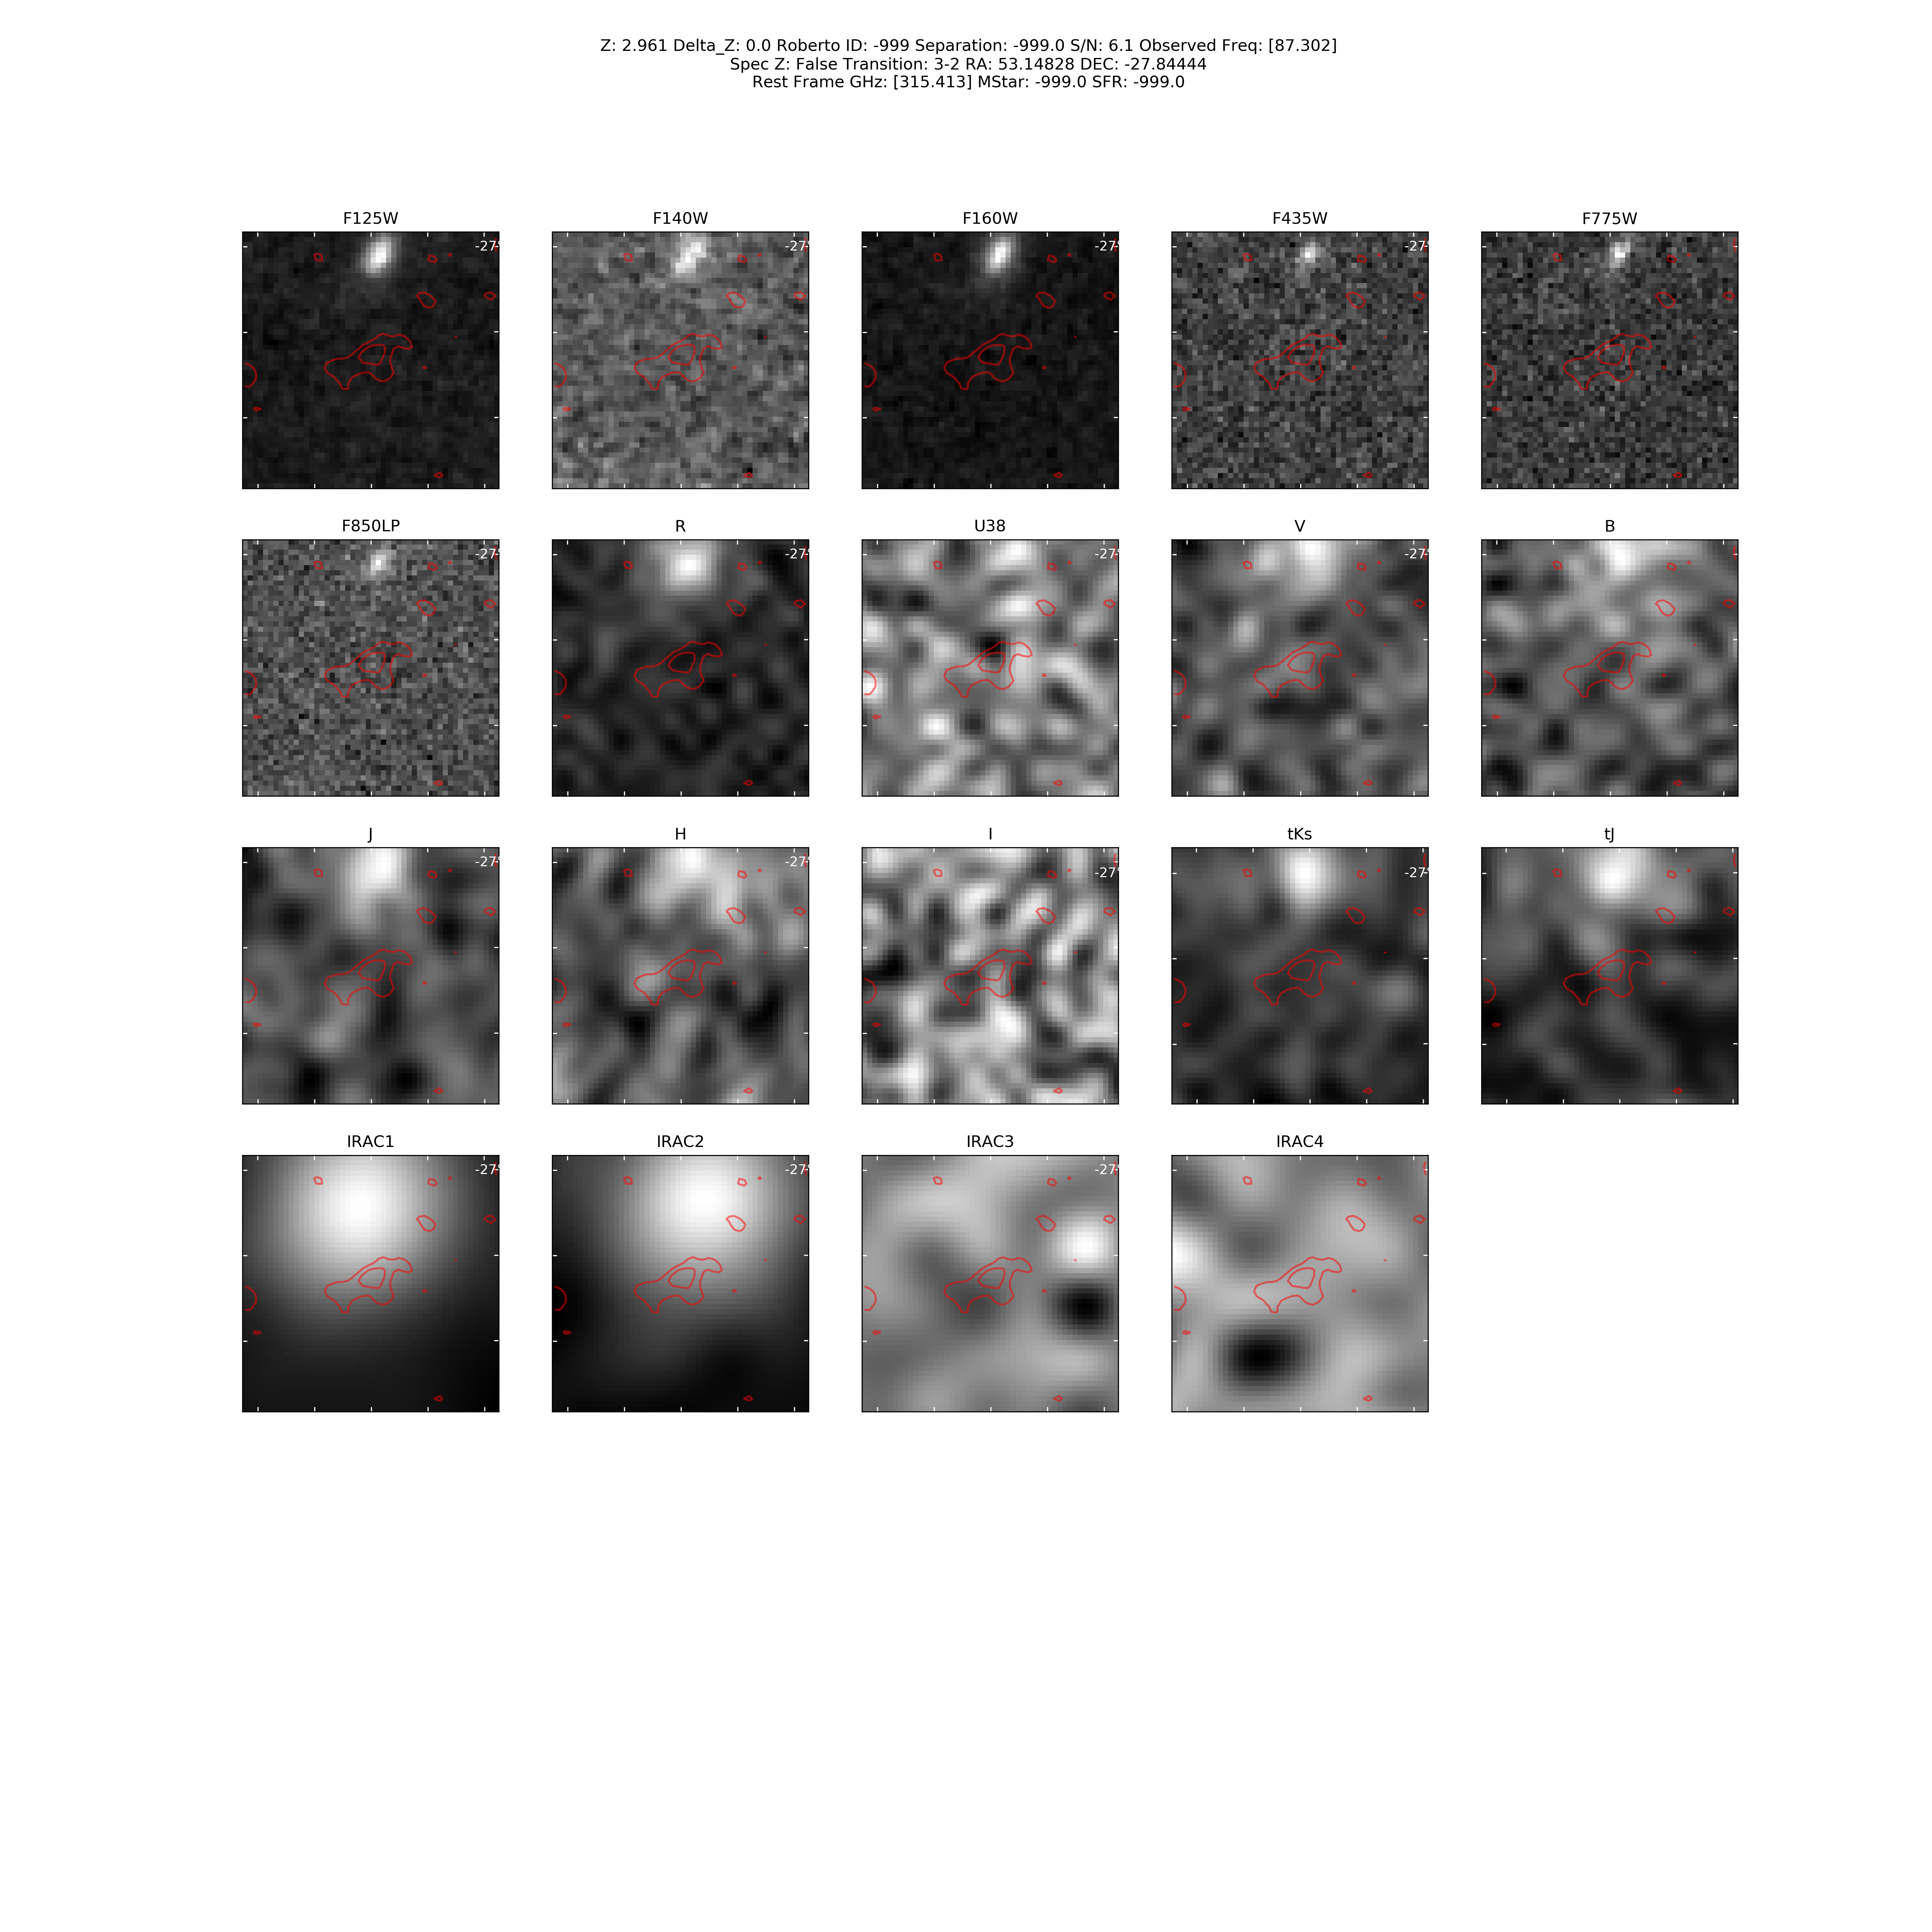
\includegraphics[width=160mm]{Matched/ASPECS_Cutout_34.png}
\caption{ID.35. Same contours and cutout size as for \ref{fig:Match_One}.}
\label{fig:Match_Three}
\end{figure}
